%dont over state the results 
%tone to use is results indicate that blaaa seems to impact
%indication of probable dependency of bla on bla
\chapter{Results}

\section{Pilot Survey and Focus Group}

\subsection{Pilot Survey Results}
As mentioned previously, the pilot survey was conducted using 14 subjects who were classed as highly aware of SLEs. The results from the pilot survey and focus group were used to improve the data collection design of the main survey. Figure 5.1 displays the results from the determination of awareness conducted on the pilot subjects.
\paragraph{}

\begin{figure}[H]
    \centering
    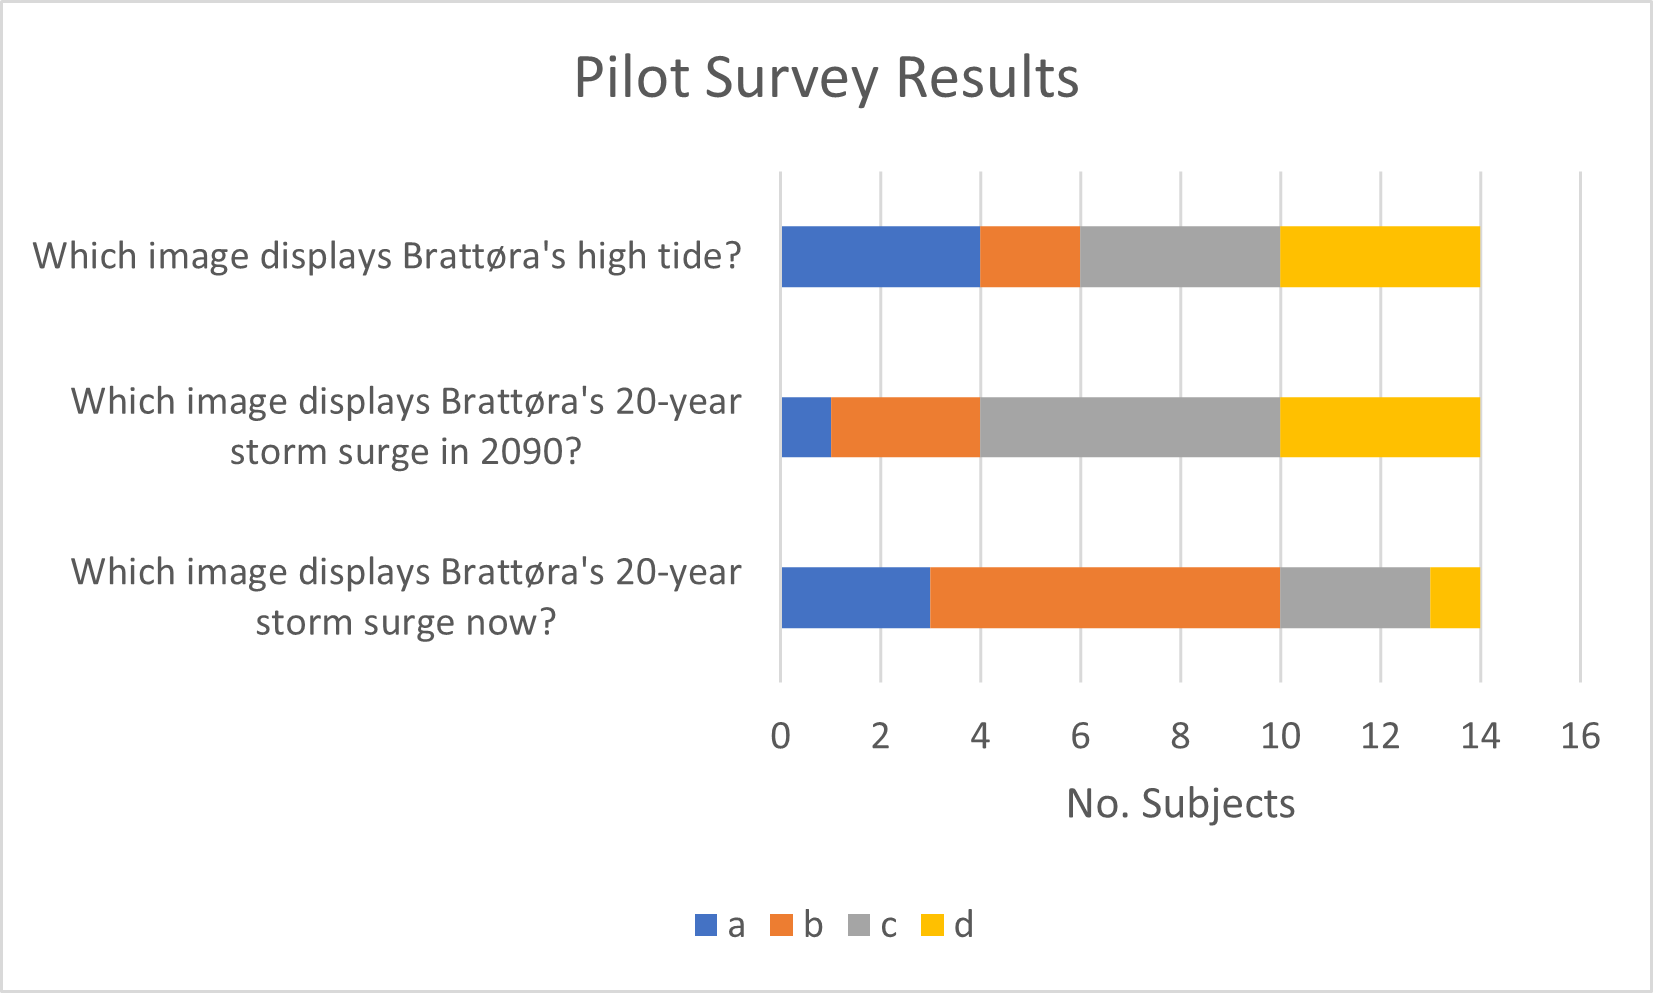
\includegraphics{fig_results/pilot_survey_results.png}
    \caption{Chart of Pilot Survey Results - 14 subjects asked three questions about SLEs. Answers are colour coded: \textit{a} is blue, \textit{b}is orange, \textit{c} is grey and \textit{d} is yellow. Response to the first question show no observable preference for any of the answers, the correct answer was \textit{c}. The second questions had a preference for answer \textit{c}, the correct answer was\textit{b}. The third question has a preference for answer \textit{b}, the correct answer was {b}.}
    \textcolor{red}{Stacked bar chart of Pilot Survey Results - 14 subjects were asked the three questions 1), 2), 3) about their perception of SLEs at the Brattøra's site. Answers are colour coded: \textit{a}: HERE YOU NEED TO ADD WHAT a MEAN! is represented in blue, \textit{b}: HERE YOU NEED TO ADD WHAT b MEAN! is represented in orange, \textit{c}: HERE YOU NEED TO ADD WHAT c MEAN! is represented in grey and \textit{d}: HERE YOU NEED TO ADD WHAT d MEAN! is represented in yellow. Response to the first question show no observable preference for any of the answers, showing a lower rate for answer \textit{b}, the correct answer was \textit{c}. The second questions had a preference for answer \textit{c}, the correct answer was\textit{b}. The third question has a preference for answer \textit{b}, that was indeed the correct answer.}
    \label{fig:pilot_survey_results}
\end{figure}

Answers corresponding with models from \cite{kartverket_se_2020} are considered to be correct in this context. For the question "Which image displays Brattøra's high tide?" the answer is C (grey), the responses for this question were widely spread over the four options. For the question "Which image display's Brattøra's 20-year storm surge in 2090? the answer is B (orange) and only 4/14 subjects selected that answer. For the question "Which image display's Brattøra's 20-year storm surge now?" the correct answer is B (orange) and half of the subjects chose this answer. 
\paragraph{}


\subsection{Focus Group Results}
The main result from the focus group  was that the maps looked too similar, especially when using smart phones for survey completion, \textcolor{red}{and it was too hard to recognize the increase of the waterline changes}. It was difficult to tell the maps apart due to the relatively small changes in the waterline. This was particularly the case for the question about the high tide. Furthermore, several participants highlighted that they did not think of SLEs in terms of area flooded, but solely in terms of changing height. This one dimensional view was highlighted by the group as a limiting factor in the understanding of potential impacts. 
\paragraph{}

When the \textcolor{red}{participants of the} focus group were asked which \textcolor{red}{type of }visualisation \textcolor{red}{method} would \textcolor{red}{be} more \textcolor{red}{effective and helpful for} [easily help] them \textcolor{red}{to }answer the questions set in the pilot survey - \textcolor{red}{between} maps, edited photographs or numerical values (see Figure 3.4 in methodology) - the majority favoured the edited photographs, but several participants favoured the numerical visualisations.
Of those that chose numeric value visualisation, there was a recognition that was likely due to their professional background, \textcolor{red}{and a previous habit of dealing with those kind of visualization method}. Those with a longer knowledge of Trondheim favoured the edited photographs. This was also highlighted as the option with the highest emotional impact and the visualisation which caught the whole focus groups attention.
\paragraph{}

\section{Technological Systems Resilience}
The results from the literature review suggest that distinguishing technological and natural systems can be difficult in a landscape which has been actively shaped by its population for so long. For Trondheim, the location of infrastructure including buildings and roads is the primary focus of the technological system which impacts resilience to SLEs. How this infrastructure is built is of course of great importance to whether a speedy return to normality is possible after a sea level extreme event. Norway has strict building regulations, with further rules about infrastructure in vulnerable locations (\cite{direktoratet_for_byggkvalitet_direktoratet_nodate}). Yet even very well designed infrastructure will still be impacted if flooded. Impacts range from the obvious  prevention of use during flooding, to post event clean up and the wear and damage which can occur from sea level extreme events.
\paragraph{}
Table 5.1 displays the number of buildings which are likely to be impacted during different SLEs in Trondheim. This is modelled by \cite{kartverket_se_2021} and was the base of later water level simulations as used in this project. Importantly, this modelling is more localised than previous models of SLEs in Norway.

\begin{table}[H]
    \centering
    \begin{tabular}{|l|l|l|l|l|}
    \hline
        \textbf{Projected SLEs }& \textbf{No. Buildings}  & ~ & ~ & ~ \\ \hline
        ~ & Private & Private & Public  & Critical  \\ \newline
        ~ & Buildings & Businesses & Buildings & Buildings \\ \hline        
        20 years return height 2022 & 160 & 77 & 10 & 0 \\ \hline
        200 years return height 2022 & 214 & 87 & 10 & 0 \\ \hline
        1000 years return height 2022 & 242 & 104 & 14 & 0 \\ \hline
        Flooded 2090 & 66 & 51 & 8 & 0 \\ \hline
        20-years return height 2090 & 264 & 119 & 17 & 1 \\ \hline
        200-years return height  2090 & 308 & 136 & 24 & 1 \\ \hline
        1000-years return height  2090 & 332 & 148 & 26 & 1 \\ \hline
        1m sea level rise & 127 & 64 & 9 & 0 \\ \hline
        2m sea level rise & 343 & 155 & 29 & 1 \\ \hline
        3m sea level rise & 584 & 285 & 55 & 3 \\ \hline
        4m sea level rise & 752 & 335 & 70 & 5 \\ \hline
        5m sea level rise & 1023 & 402 & 77 & 8 \\ \hline
    \end{tabular}
    \caption{Impact of SLEs to Buildings in Trondheim translated from \cite{kartverket_se_2021}.  }
    \label{building-impact-sle}
\end{table}


Table 5.1 shows that there is currently some risk from SLEs to buildings in Trondheim, now and in the future. For example, the projected 20 year return height - 2022 is expected to cause the flooding of 247 buildings in total. Additionally, the table shows the number of building projected to flood at different projected SLEs. The major contrast between the 20 year return height - 2022 and the 20 year return height - 2090 is that the water level is high enough to flood a critical building. Flooding of a critical building would also occur at 2m sea level rise. It is projected by 2090 that 115 building will be continuously flooded.
\paragraph{}
The number of building projected to flood increases with the projected height of sea level rise. 


\section{Natural Systems Resilience}


\section{Social Systems Resilience}

This section focuses on the results gained from the survey conducted to determine social resilience to SLEs in Trondheim.  It also includes the results from Kruskal Wallis Rank Sum Tests and Shapiro Tests. Each of the results gained from the survey questions is displayed in a graph. These results will be discussed later to determine Trondheim's social systems resilience to SLEs. The tables and graphs in the following section make reference to the main research survey questions. The full survey, in either Norwegian or English, is available in the appendix. Reference in the text is only made to the English questions. 



\subsection{Place and language}
Table 5.2 shows the by place and language splits of the 153 subjects who completed the main survey. 
\begin{table}[H]
    \centering
    \begin{tabular}{|l|l|l|l|}
    \hline
    \textbf{Place}  & \textbf{ English} & \textbf{Norwegian} & \textbf{Total Subjects}  \\ \hline
      Skansen & 11 & 18  & 29    \\ \hline
      Nidelva & 28 & 29 & 57      \\ \hline
      Grillstad & 13 & 24 & 37       \\ \hline
      Brattøra & 14 & 16 & 30     \\ \hline
      Total & 66 & 87 & 153   \\ \hline
     \end{tabular}
    \caption{Place and language subjects chose to Answer on. The most popular sub-survey was Nidelva with 57 responses, representing 37 percent of responses. Next popular was Grillstad with 37 responses and then Brattøra with 30 and Skansen with 29 respectively. The reasonable spread of response does allow for comparison. More subjects responded in Norwegian (87) than English (66), but it was comparably split for each location whether the survey was completed in Norwegian or English. }
    \label{tab:place}
\end{table}
\paragraph{}

The most popular place for responses was Nidelva, followed by Grillstad, Brattøra and finally Skansen. Almost evenly split for each location was whether the survey was completed in Norwegian or English. Overall responses in English totalled 66, while the Norwegian survey had 87 responses.  

\subsection{Interest Level in SLEs}
The following two figures show the results from the survey questions on self-ranking interest level.  Figure 5.10 shows the split across the five levels of interest. 80 percent of subjects responded with a medium or higher level of interest. 


\begin{figure}[H]
    \centering
    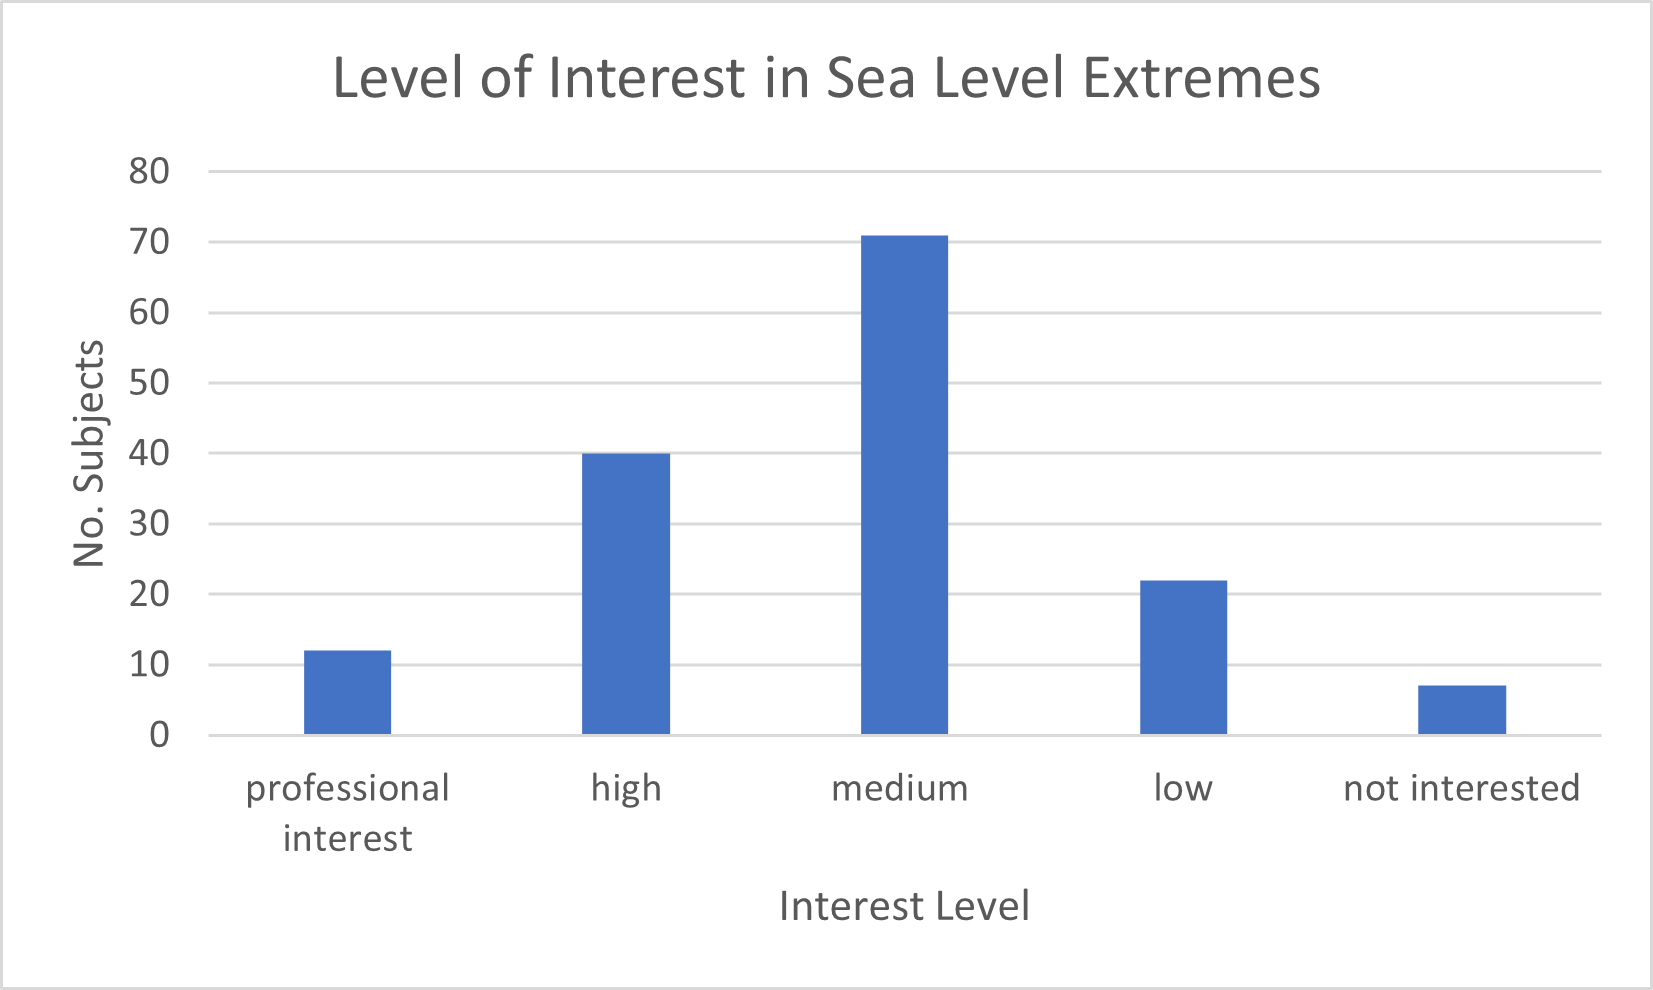
\includegraphics{fig_results/interest-level.png}
    \caption{Interest Level in SLEs - There is a good spread in the results to this question. 22 subjects have low interest in SLEs, 7 are not interested.  Almost half of the subjects (71/153) answered that they have a medium interest in SLEs. More subjects answered that they had a high level of interest (40) than have a low level of interest in SLEs. 12 subjects answered that they have professional interest in SLEs. }
    \label{fig:my_interest_level}
\end{figure}
\paragraph{}

The majority of subjects answered that their interest in SLEs is medium. Interestingly, 7 subjects responded that they have no interest. 12 subjects responded that they have a professional interest in SLEs. 
\paragraph{}
Figure 5.11 displays awareness against self-ranking interest level.

\begin{figure}[H]
    \centering
    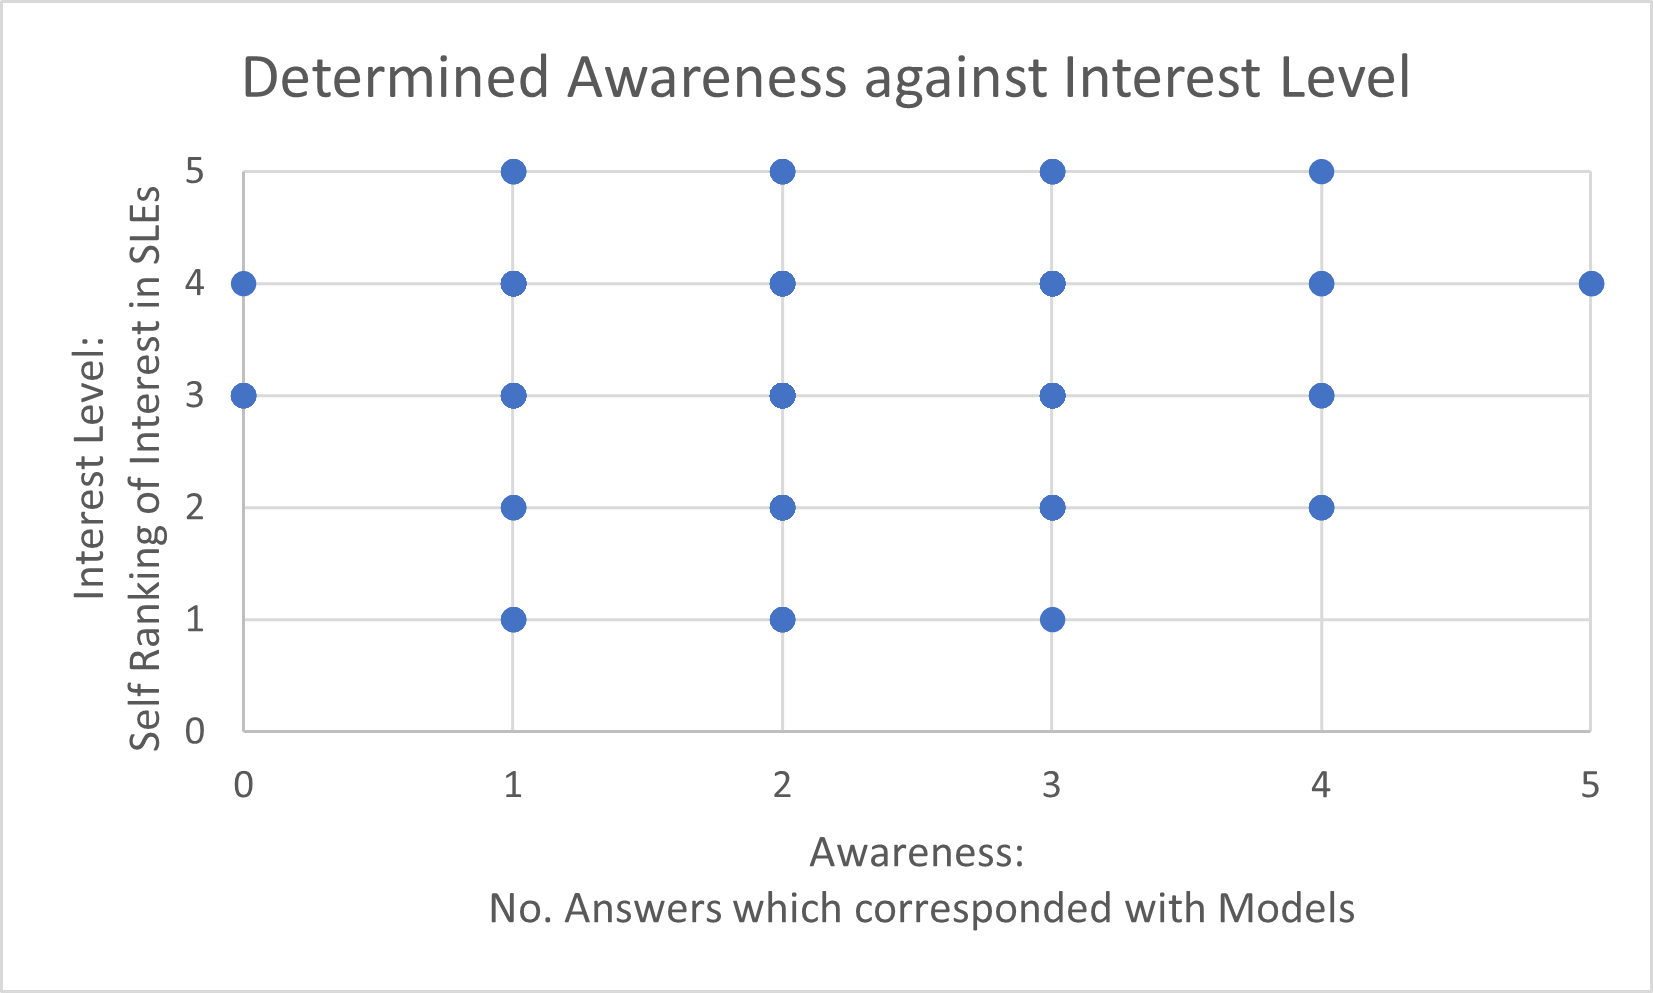
\includegraphics{fig_results/aware_vs_interest.png}
    \caption{Determined Awareness Against Interest Level -  Professional interest is level 5 on the y-axis, High  is level 4, medium is level 3, 2 is low interest and 1 is not interested. Subjects who responded high levels of interest are determined as representing all levels of awareness.}
    \label{fig:aware_vs_interest}
\end{figure}
\paragraph{}

There is no linearity or other pattern observed in Figure 5.11. Medium level self ranking of interest has almost as broad a variation as high level, but does not include any subjects who were determined to have the highest level of awareness.  It is worth noting  that Figure 5.11 does not display how often subjects interest level matched their awareness. A single subject is enough for a blue dot to be displayed as there is no weighting with this Figure, though this can be inferred from figure 5.10. 


\subsection{Memory of SLEs and Length of Place-based Knowledge}
The spread of the memory of sea level extreme events in Trondheim by the subjects is shown in figure 5.12.

\begin{figure}[H]
    \centering
    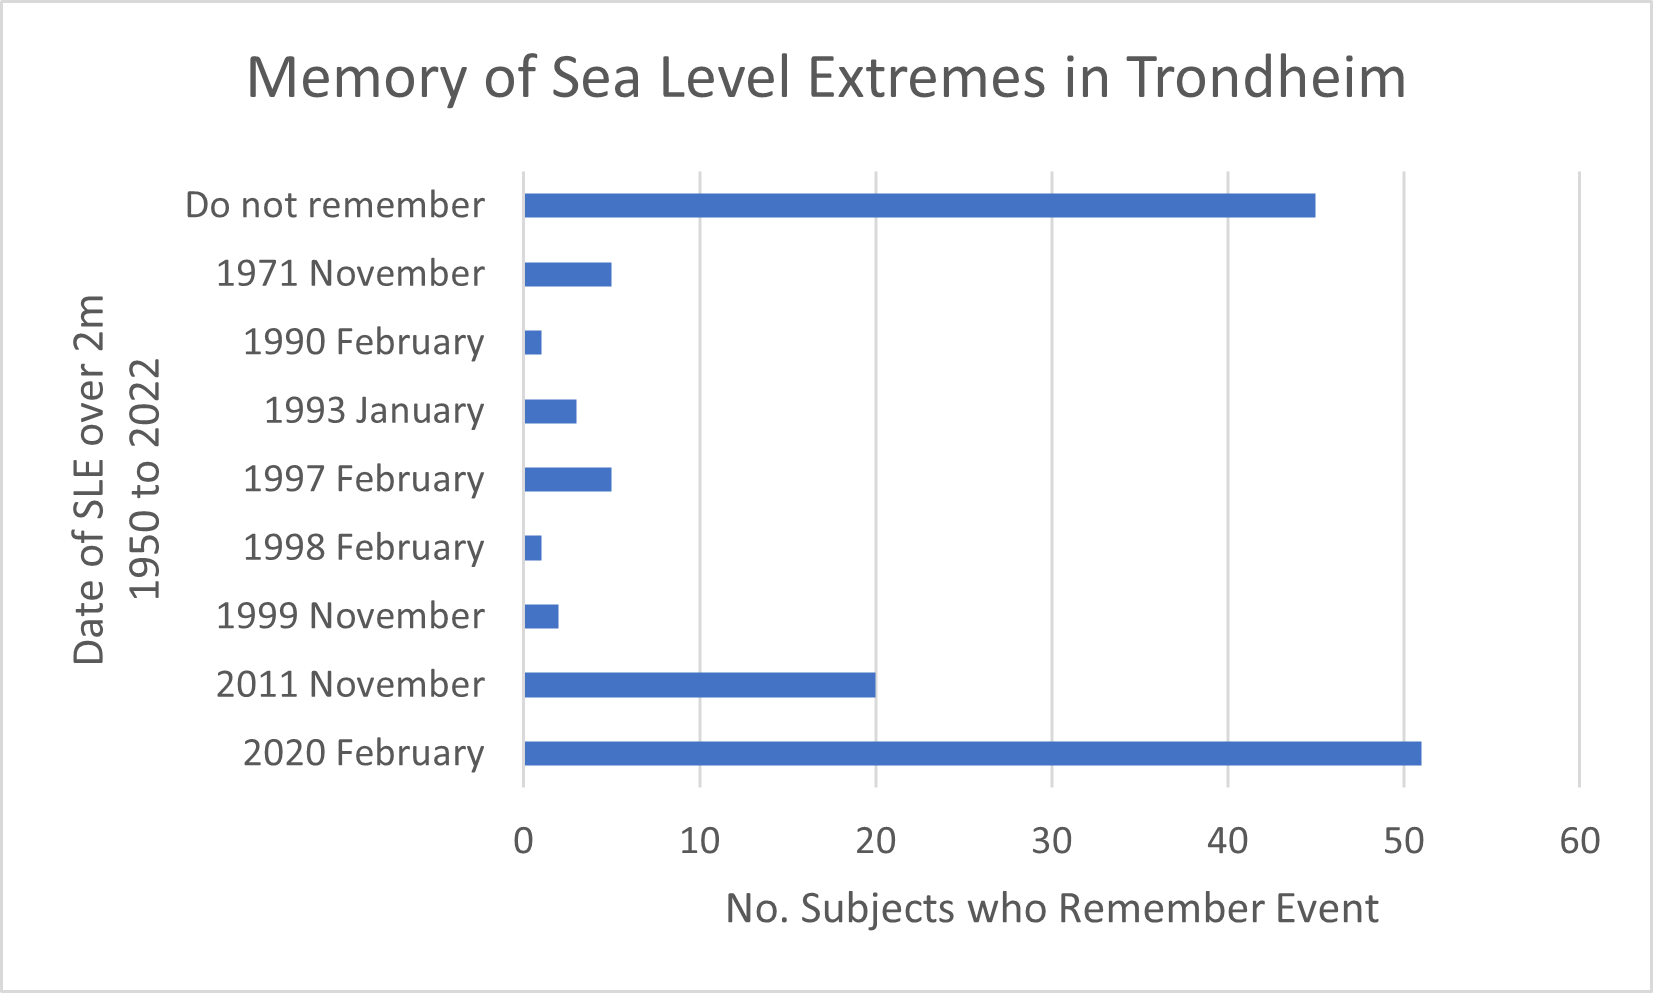
\includegraphics{fig_results/memory-sle.png}
    \caption{Memory of SLEs - The subjects were asked which about each sea level extreme event (water level higher than 2m) they remembered occurring between 1950 and summer 2022. For the full list of potential events please consults the relevant question in the appendix. 45 out of 153 subjects do not remember any sea level extreme event in Trondheim. Only one subject remembered every sea level extreme event dating back to 1950 in Trondheim. 51 subjects remembered the sea level extreme event in February 2020. }
    \label{fig:my_label}
\end{figure}
\paragraph{}

Memory is a very skewed factor. 30 percent of subjects have no memory of SLEs in Trondheim. Once that answer is excluded, there is almost an exponential increase in the number of subjects who remember the event the closer to the present. 
\paragraph{}
Figure 5.13 shows the responses to the place-based length of knowledge question.

\begin{figure}[H]
    \centering
    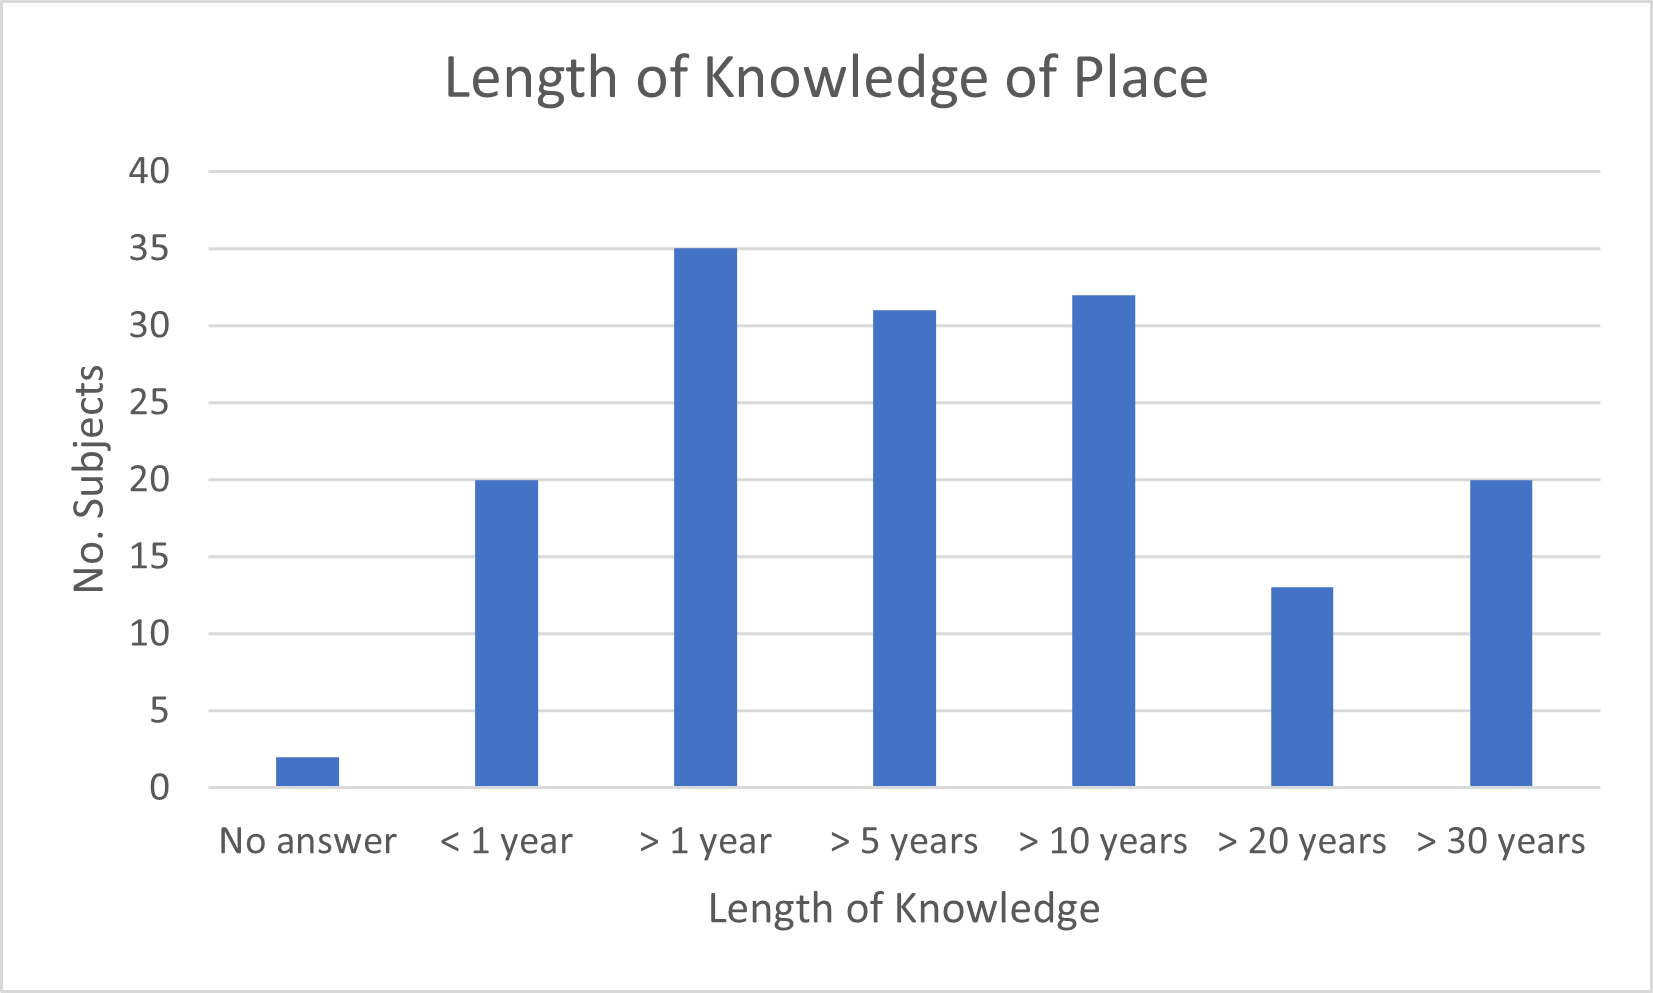
\includegraphics{fig_results/long_know.png}
    \caption{Length of Knowledge of Subjects. 96 subjects had a length of knowledge about the place greater than 5 years 35 subjects had length of knowledge less than 5 years, but more than 1. Only 20 respondents had a length of knowledge under 1 year}
    \label{fig:long_know}
\end{figure}

20 subjects responded that they had a length of knowledge of Trondheim under one year. 96 subjects responded that they had a length of knowledge greater than five years, which includes the sea level extreme event occurring in February 2020, which only 51 subjects remembered. The difference between a sea level extreme event and a disaster and how this impacts memory and resilience is expanded upon in the discussion.


\subsection{Information Access about Climate and Place}
There is significant skew in how subjects access information about climate and place as can be seen in Table 5.3 and Table 5.4 below. That individuals with a broader range of information sources have higher levels of awareness is one of the hypotheses outlined in the introduction. 

\begin{center}
\begin{table}[H]
    \centering
    \begin{tabular}{|l|l|l|l|l|l|l|}
    \hline
        \textbf{Factor} & \textbf{mean} & \textbf{Std Dev}. & \textbf{ min} & \textbf{max} & \textbf{ range} & \textbf{skew}  \\ \hline
        
      Sum of Information Access & 3.50 & 1.72 & 0 & 8 & 8 & 0.24  \\ \hline
        Personal Observation  & 0.45 & 0.50 & 0 & 1 & 1 & 0.20 \\ \hline
        Family & 0.18 & 0.38 & 0 & 1 & 1 & 1.68  \\ \hline
        Friends & 0.23 & 0.42 & 0 & 1 & 1 & 1.28  \\ \hline
        Newspapers & 0.72 & 0.45 & 0 & 1 & 1 & -0.96 \\ \hline
        TV & 0.46 & 0.50 & 0 & 1 & 1 & 0.14 \\ \hline
        Social Media & 0.63 & 0.48 & 0 & 1 & 1 & -0.55 \\ \hline
        Membership of Organisations & 0.14 & 0.35 & 0 & 1 & 1 & 2.09 \\ \hline
       Peer Reviewed Publications & 0.39 & 0.49 & 0 & 1 & 1 & 0.44 \\ \hline
        Formal Education & 0.29 & 0.46 & 0 & 1 & 1 & 0.89 \\ \hline
        
         \end{tabular}
    \caption{Information about Climate Summary Statistics information access}
\label{table:summary_stats_info_access}
\end{table}
\end{center}

\begin{center}
\begin{table}[H]
    \centering
    \begin{tabular}{|l|l|l|l|l|l|l|}
    \hline
         \textbf{Factor} & \textbf{mean} & \textbf{Std Dev.} & \textbf{min} & \textbf{max} & \textbf{range} & \textbf{skew}  \\ \hline
        Sum of Information Access & 1.94 & 1.34 & 0 & 8 & 8 & 1.61 \\ \hline
        Personal Observation & 0.73 & 0.45 & 0 & 1 & 1 & -1.00  \\ \hline
        Family & 0.10 & 0.31 & 0 & 1 & 1 & 2.56 \\ \hline
        Friend & 0.19 & 0.39 & 0 & 1 & 1 & 1.57  \\ \hline
        Newspaper & 0.35 & 0.48 & 0 & 1 & 1 & 0.64  \\ \hline
        TV & 0.14 & 0.35 & 0 & 1 & 1 & 2.09 \\ \hline
       Social Media & 0.33 & 0.47 & 0 & 1 & 1 & 0.73  \\ \hline
        Membership of Organisations & 0.04 & 0.19 & 0 & 1 & 1 & 4.70 \\ \hline
        Trondheim Municipality & 0.07 & 0.26 & 0 & 1 & 1 & 3.28\\ \hline
                
         \end{tabular}
    \caption{Information about Place Summary Statistics information access}
\label{table:summary_stats_info_access}
\end{table}
\end{center}

 Social media is a more common response for information about climate than information about place. Membership of organisations is the least popular response for both information about climate and place. Personal observation is the most popular response for information about place and the fourth most popular response for information about climate. On average, subjects selected more sources for information about climate than information about place. 
\paragraph{}
This highly skewed responses with a large variation in mean and standard deviation impacts the type of hypothesis testing which could be carried out.

\subsection{Community Membership}
Subjects were self-selecting stakeholders.  As stated in the methods, they were asked to identify themselves as members of communities that were highlighted by a stakeholder analysis. They were also given the choice to write in other community membership if they selected other. Figure 5.14 displays the community memberships selected by the subjects. 

\begin{figure}[H]
    \centering
    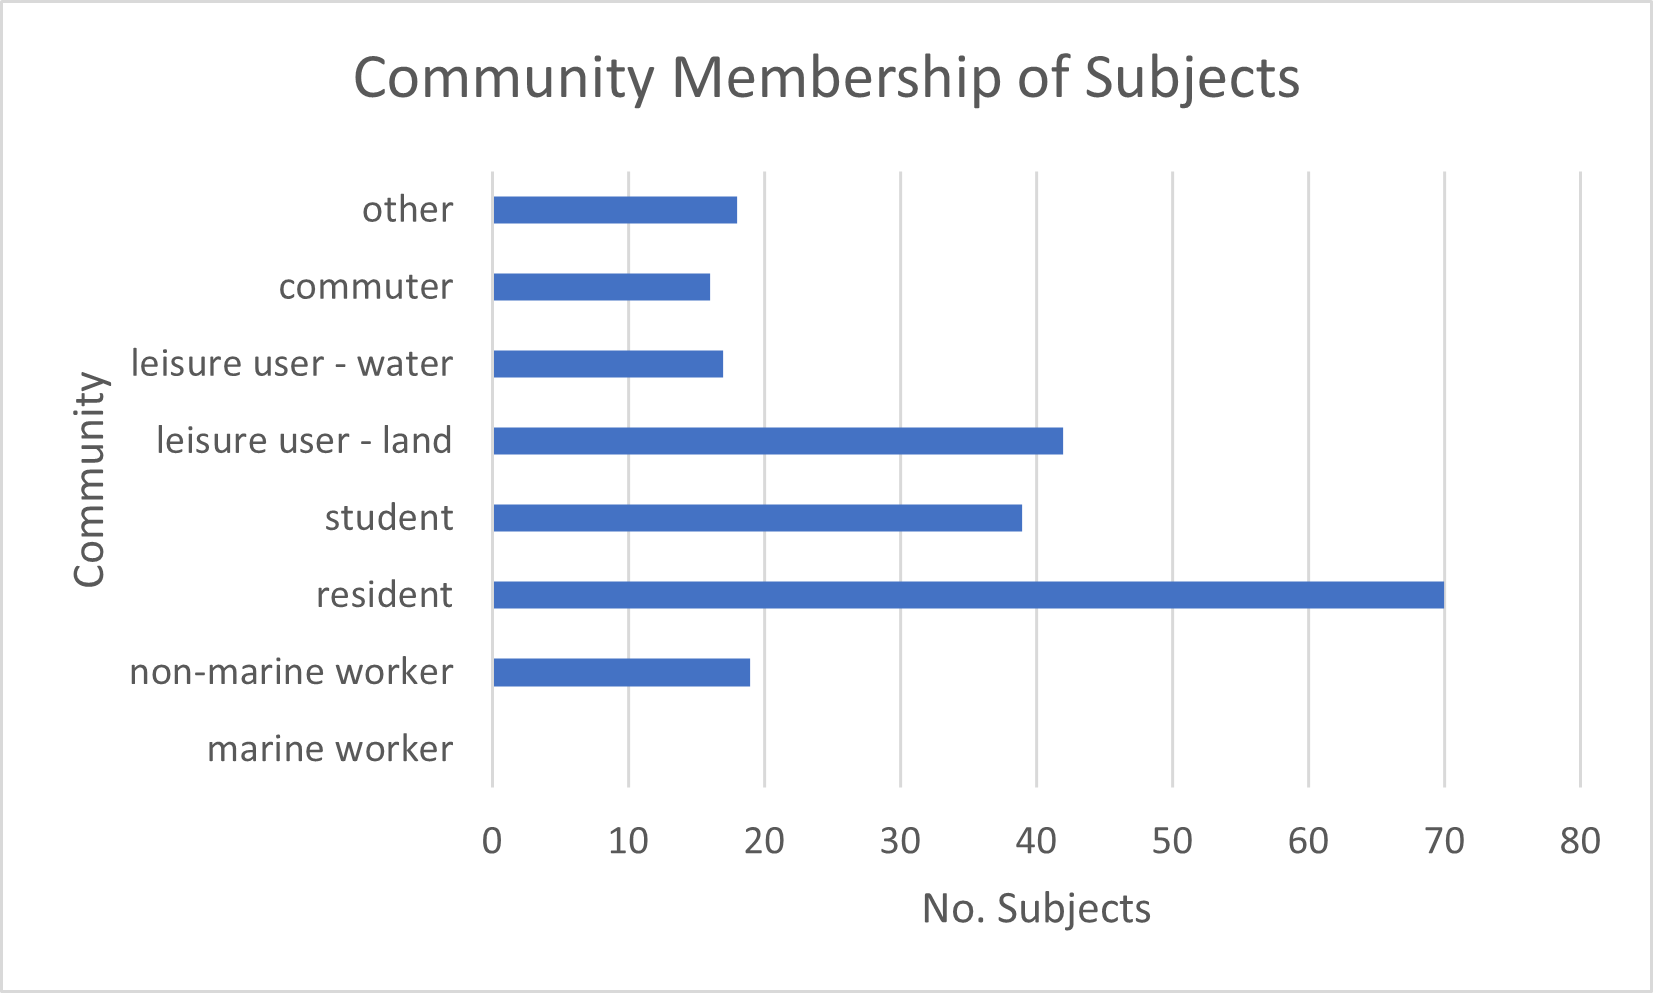
\includegraphics{fig_results/com-mem-horizontal.png}
    \caption{Membership of Communities. There were 221 selections done by the 153 subjects. However many subjects only selected one community. The most selected community was resident, however only 70 out of 153 subjects - under half. }
    \label{fig:my_label}
\end{figure}
\paragraph{}

There are 70 subjects who answered that they are residents. This is the most common choice. Interestingly, very few subjects who answered they were students also selected a second community membership. Subjects who answered as other were either visitors, tourists or sailors. That subjects only ticked one box in the survey means it is unlikely that they responded with every community that they are part of, just the identity they feel is most important. No subjects responded as marine workers. This impact of subjects only selecting a single response in these types of questions and the impact it has is discussed further in the discussion of framework. 


\subsection{Access to Survey. }
Figure 5.15 shows how subjects accessed the survey.  

\begin{figure}[H]
    \centering
    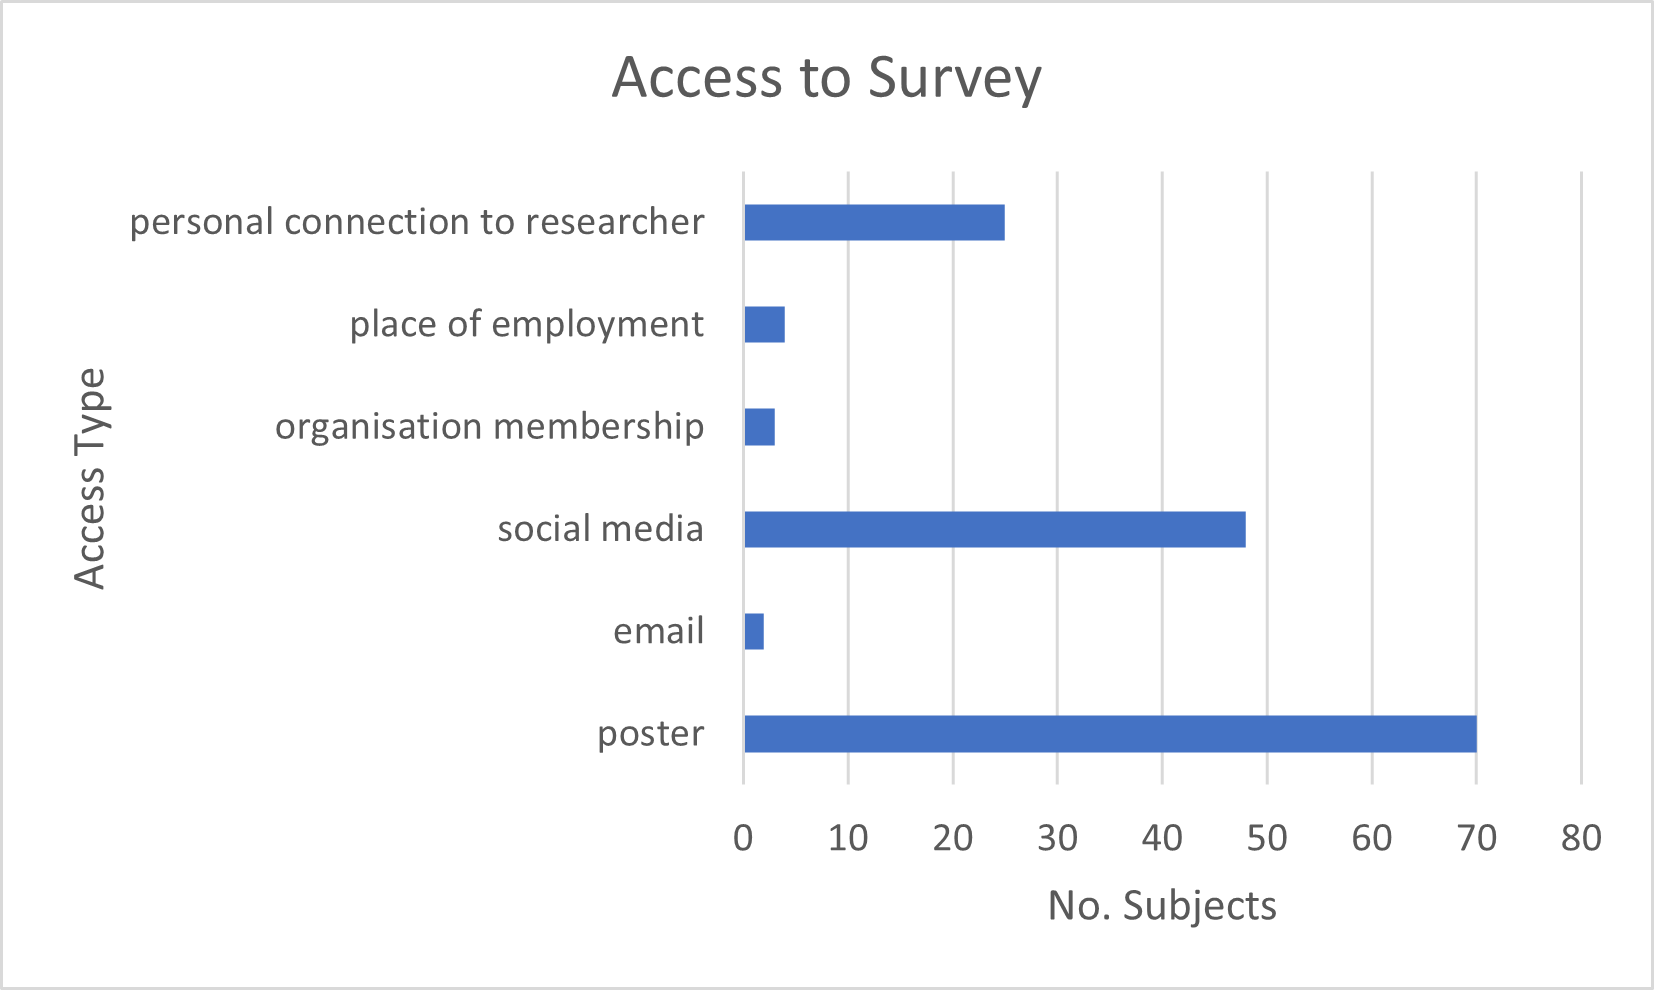
\includegraphics{fig_results/access_survey.png}
    \caption{Access to Survey - Six access types were included and the number of subjects who chose each is shown. }
    \label{fig:my_label}
\end{figure}
\paragraph{}


The most common access method of the survey was poster, with 70 subjects selecting this choice. This is followed by social media which has 47 subjects choosing this. 25 subjects accessed the survey due to personal connection to researcher. Accesses via email, place of employment and organisation membership are all under 10. Subjects could chose more than one access type. For example, a subject could have accessed via personal connection to researcher and social media, due to the researcher sharing this survey on their personal social media.  
\paragraph{}



\subsection{Perceived Risks}
Figure 5.16 shows the  number of responses selecting a perceived risk to infrastructure. Figure 5.17 shows the number of responses selecting a perceived risk to people. .

\begin{figure}[H]
    \centering
    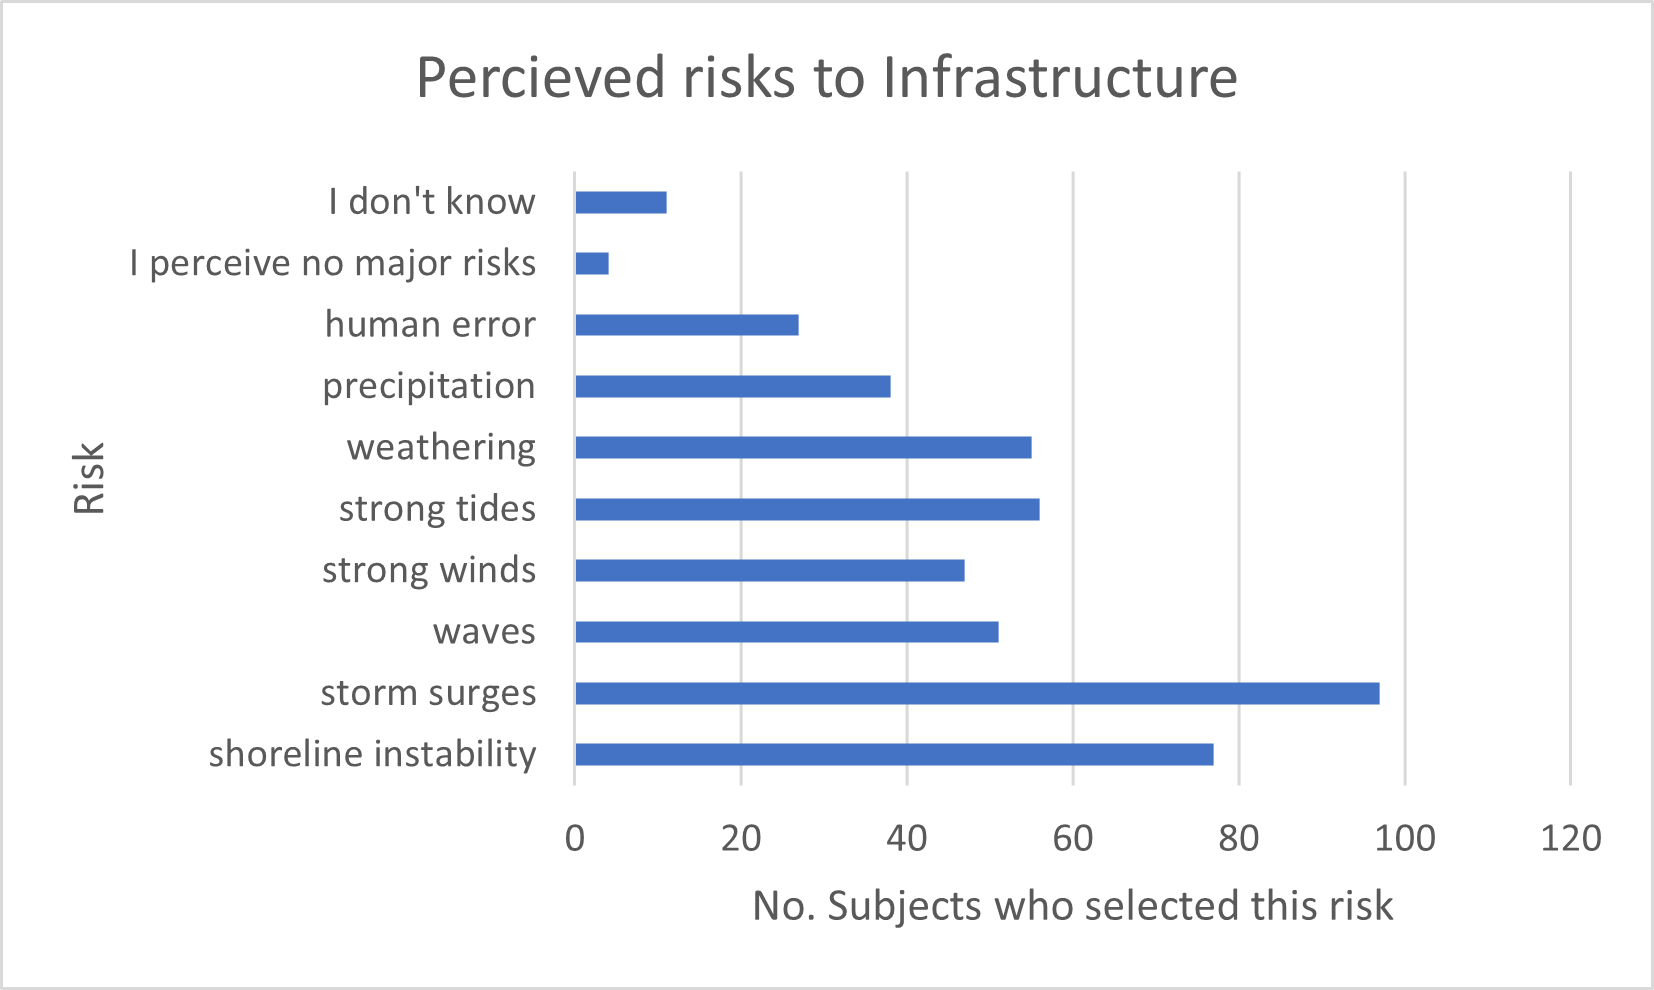
\includegraphics{fig_results/percieved risks to infrastructure.png}
    \caption{Perceived risks to Infrastructure Risks - 97 subjects selected storm surges as a risk to infrastructure. Only 4 subjects responded that they perceived no major risks to infrastructure and 11 subjects responded that they don't know. Human error was only selected by 27 subjects making it the risk the least number of subjects were concerned about. There is greater perception of weather impacts on infrastructure with 47 subjects highlighting strong winds, 51 subjects selecting waves, 56 subjects selecting strong tides and 38 selecting precipitation. After storm surges which were mentioned multiple times in the survey there is a perception of shoreline instability with 77 subjects selecting it as a risk to infrastructures.   }
    \label{fig:my_label}
\end{figure}
\paragraph{}





\begin{figure}[H]
    \centering
    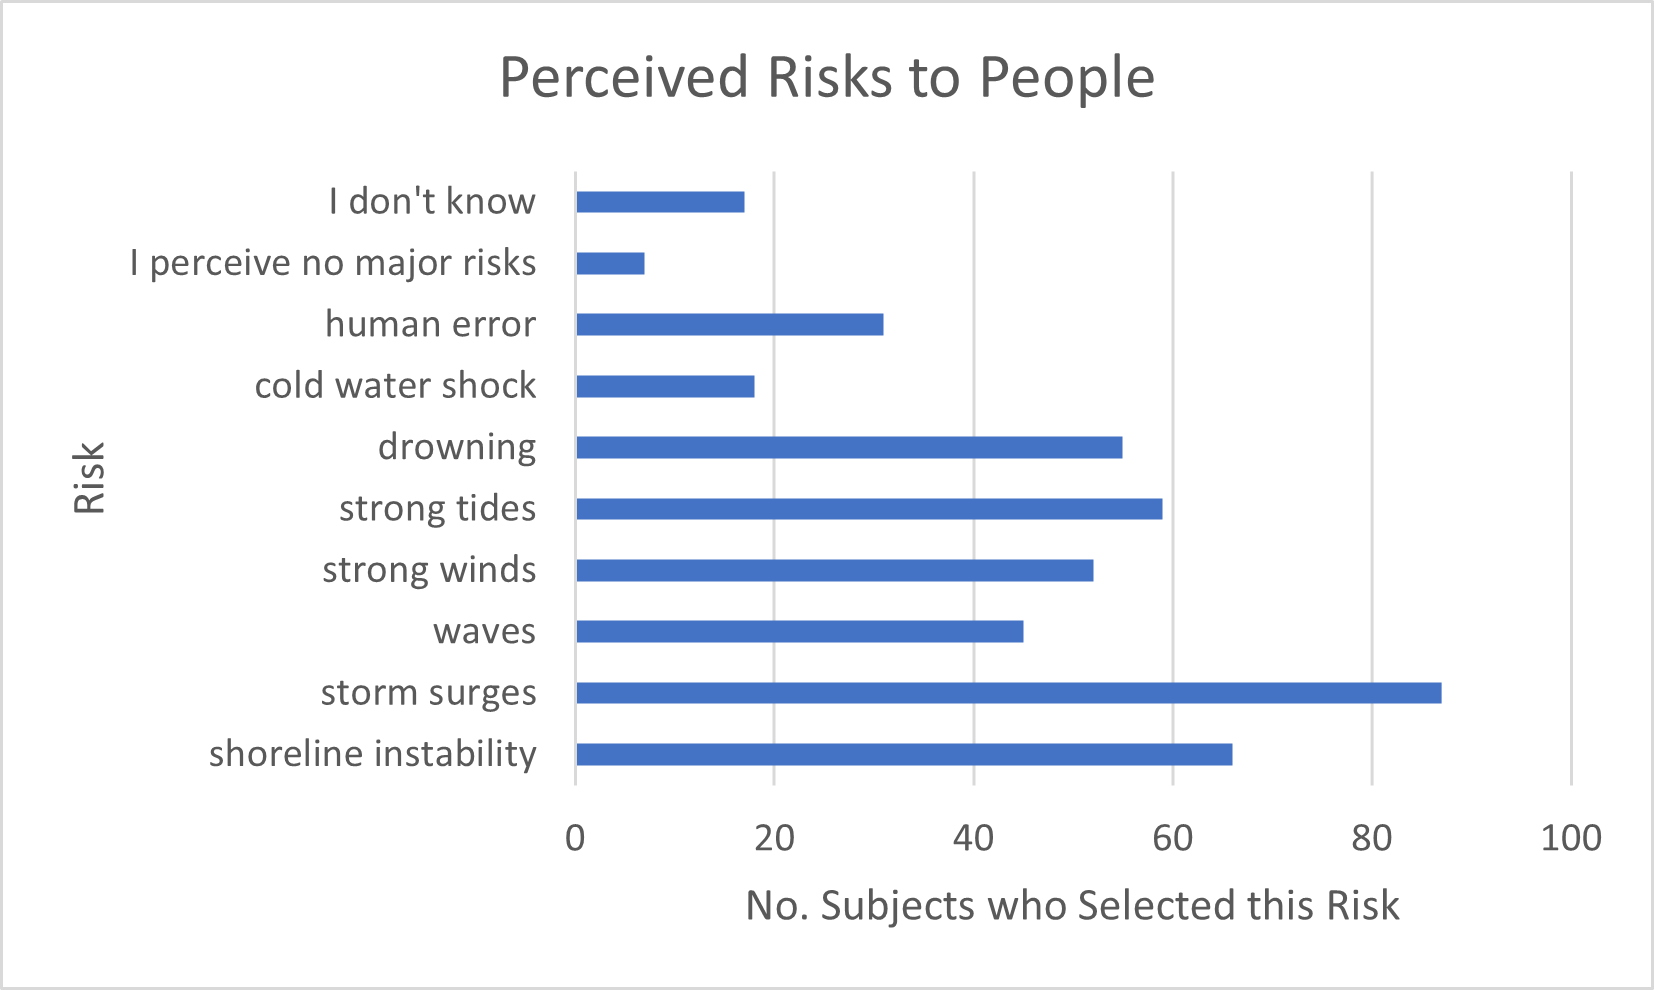
\includegraphics{fig_results/percieved risks to people.png}
    \caption{Perceived risks to People. 66 subjects selected that they perceive storm surges as a risk to people in the research sites. }
    \label{fig:my_label}
\end{figure}
\paragraph{}
It is interesting that more than 80 subjects have selected storm surges as a risk to infrastructure or people. Shoreline instability is also a very common response across both questions. It is notable that the vast majority of subjects do identify risks to people and infrastructure for these places when offered answers. The response of "I don't know" is more common that the "I percieve no major risks". 


\section{Determination of Subjects' Awareness}
Figure 5.18 shows that the subjects displayed a high awareness of the tides in Trondheim. 

\begin{figure}[H]
    \centering
    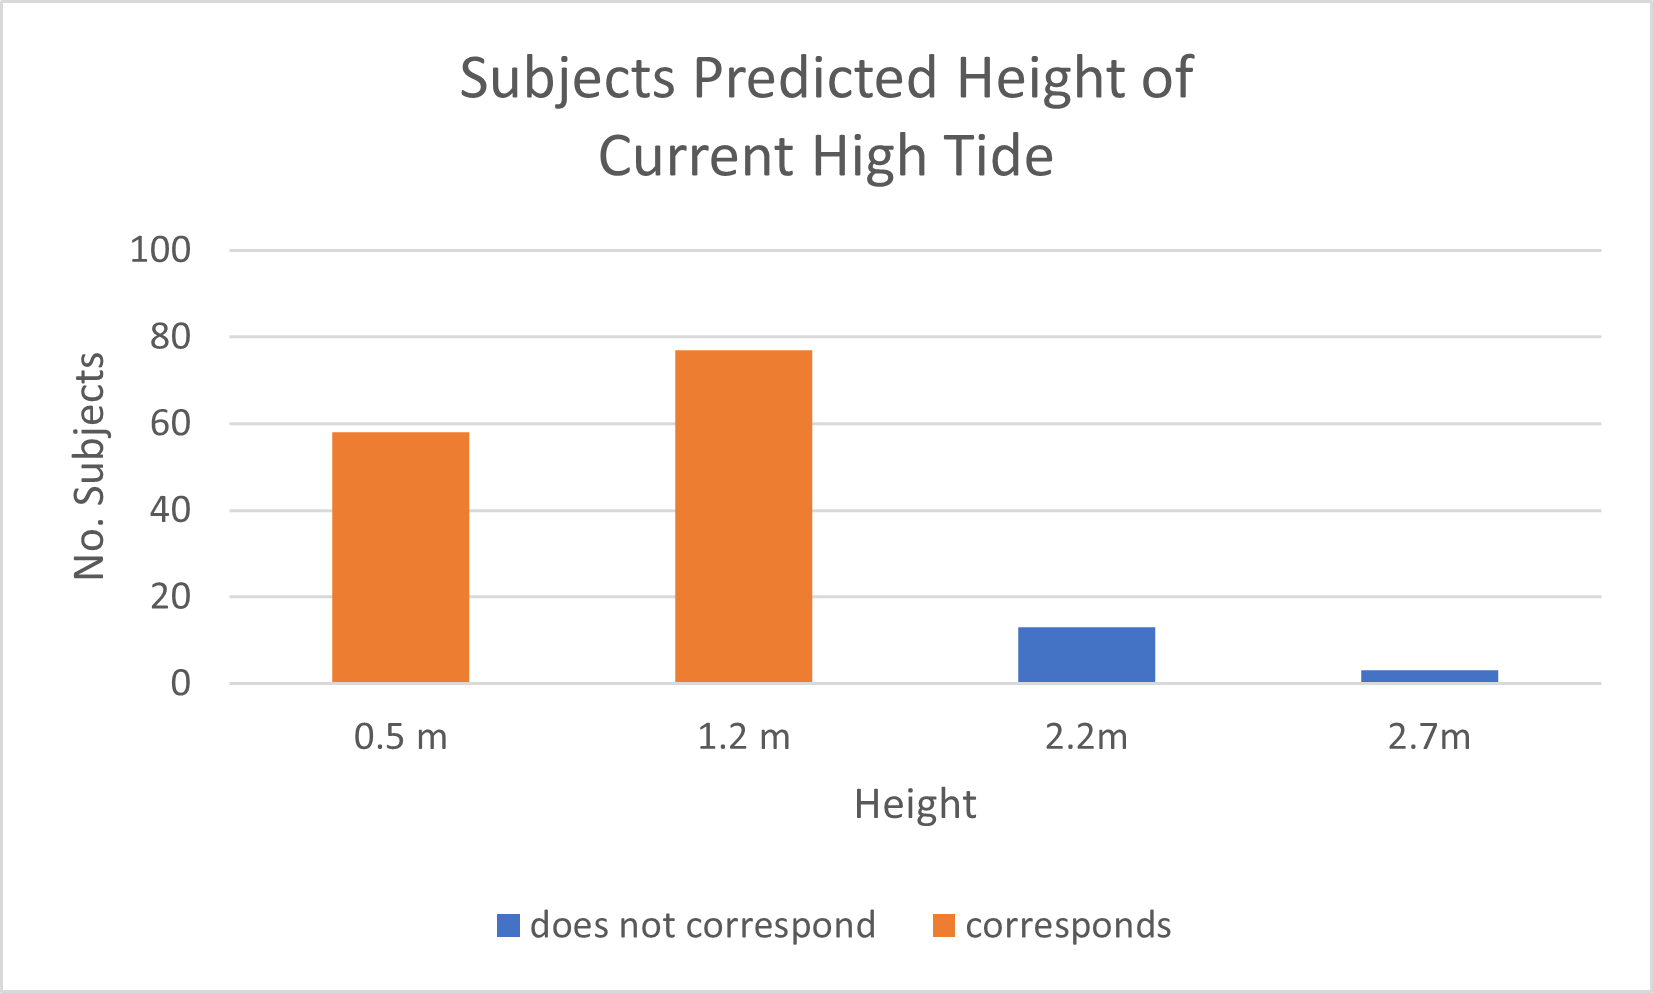
\includegraphics{fig_results/2022-hightide-answers.png}
    \caption{Subjects Predicted Height of Current High Tide. Height 0.5m is the neap high tide, Height 1.2m is the Spring High Tide. The vast majority of subjects selected an answer which corresponds with models of tides in Trondheim. Under 20 subjects responded with an answer which does not correspond with models of tides. 58 subjects chose 0.5m, 77 subjects chose 1.2m meaning that 135 out of 153 subjects, 88 percent chose what could be considered the correct answer for high tide. Only 13 subjects chose 2.2m and 3 subjects chose 2.7m}
    \label{fig:high-tide-answer}
\end{figure}
\paragraph{}

The height chosen largely corresponds with either the spring or neap high tide - over 80 percent of subjects chose a value which corresponds with the models from \cite{kartverket_se_2020}. Under 20 subjects responded with an answer which does not reflect the models from \cite{kartverket_se_2021}. 
\paragraph{}
Figure 5.19 shows the responses to the question on the predicted height of the current 20 year storm surge. 
\begin{figure}[H]
    \centering
    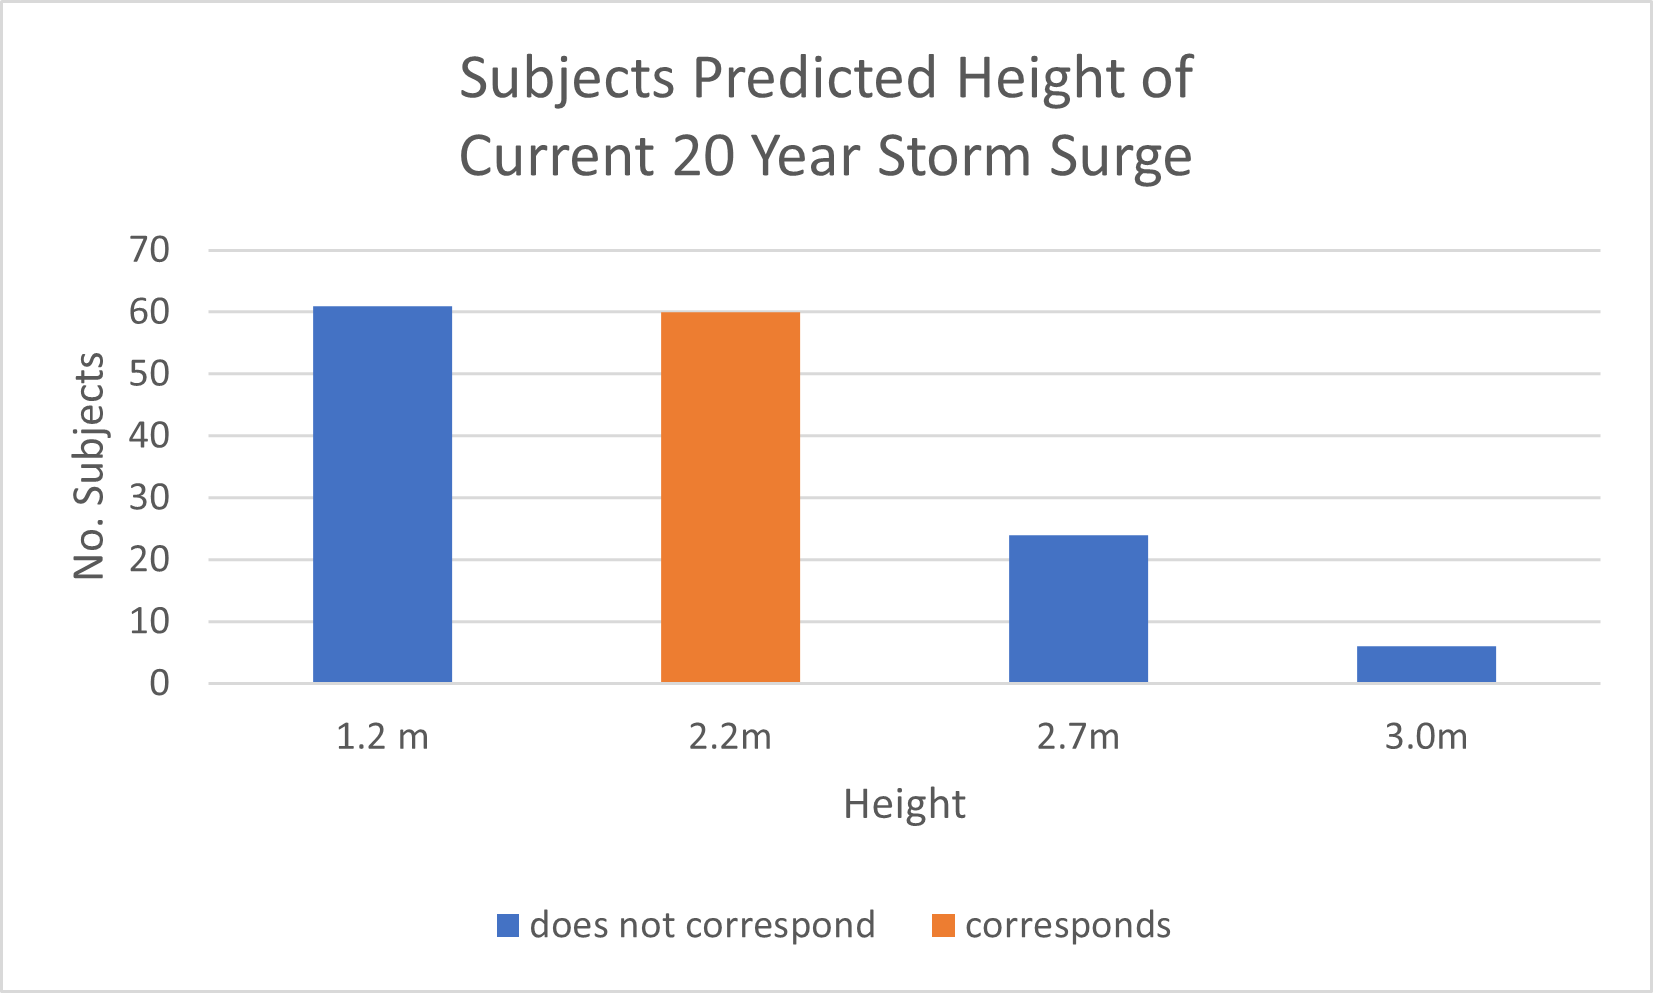
\includegraphics{fig_results/2022-20yrss-answer.png}
    \caption{Subjects Predicted Height of Current 20 Year Storm Surge. 61 subjects chose 1.2m this is very comparable to the 60 which chose 2.2m which is the answer which corresponds with \cite{kartverket_se_2021}. 24 subjects chose 2.7m and only 6 subjects chose 3.0m}
    \label{fig:2022-stormsurge-answers}
\end{figure}
\paragraph{}
The majority of subjects chose 1.2m as the predicted height of the 20 year storm surge, this does not correspond with models from \cite{kartverket_se_2021}. In fact, 1.2m is equal to the current high tide. Almost equally often chosen was the answer which does correspond with models from \cite{kartverket_se_2021}, 2.2m, with 60 subjects choosing this answer. This means that 43 percent of subjects chose the answer which corresponds with \cite{kartverket_se_2021}. Around 20 percent (30/153) of subjects chose an answer higher than the models indicate.
\paragraph{}
Figure 5.20 shows the responses to the question on the predicted height of the 2090 20 year storm surge.

\begin{figure}[H]
    \centering
    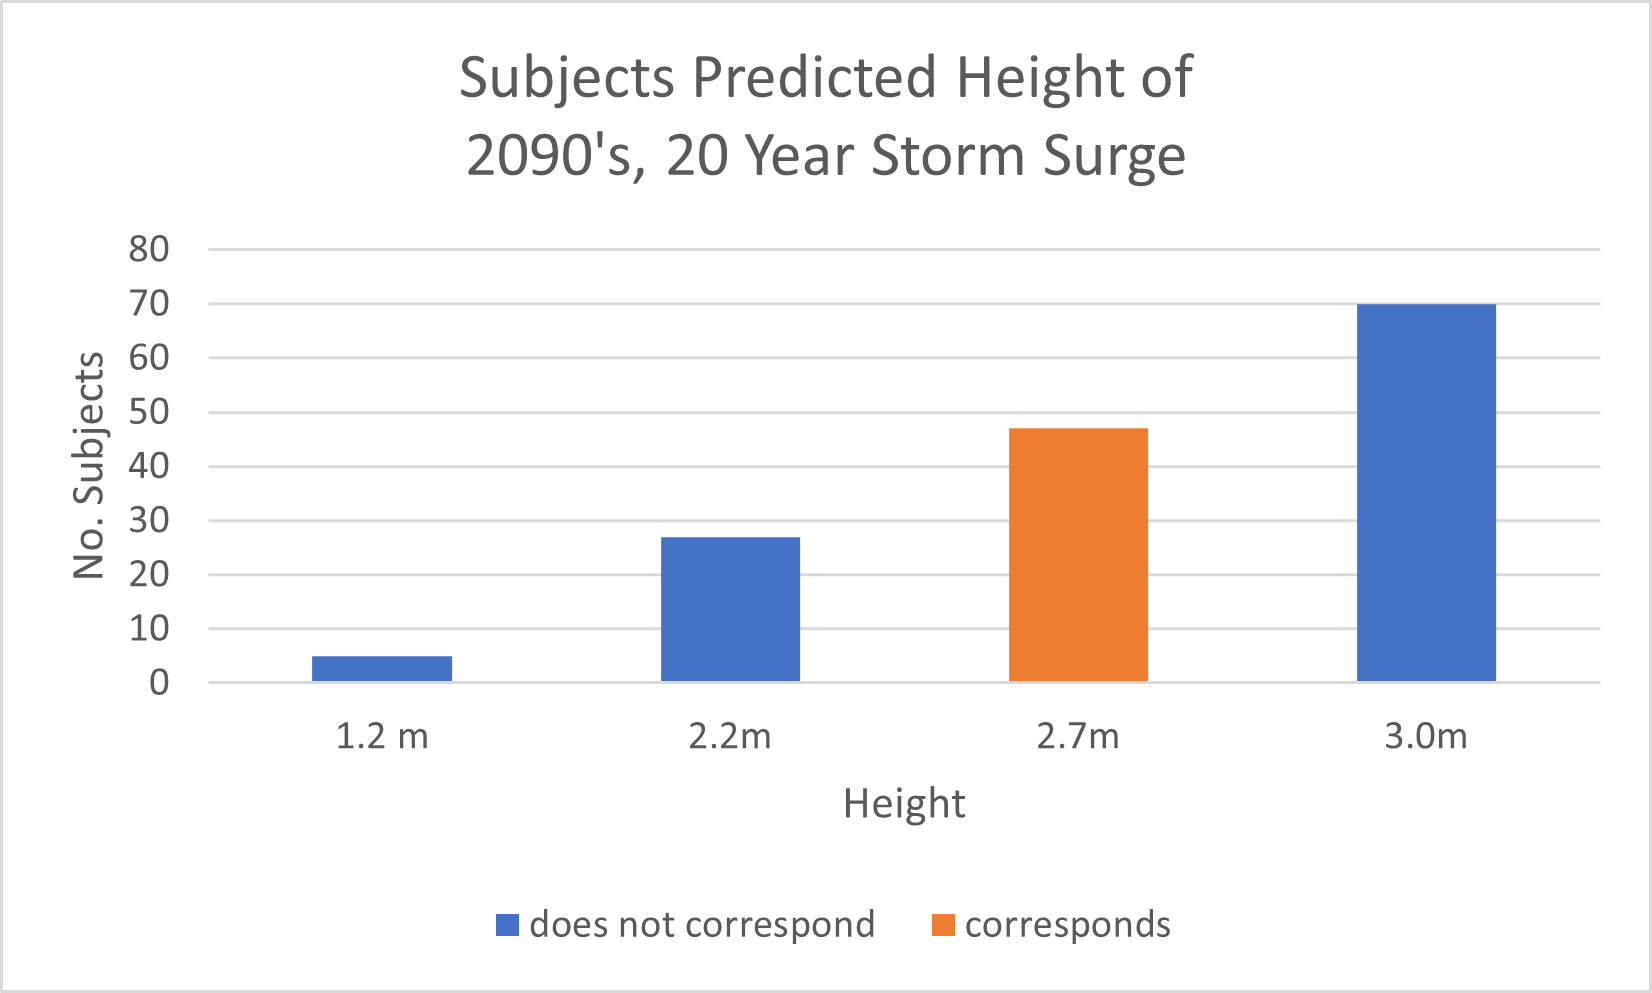
\includegraphics{fig_results/2090s 20yr ss answers.png}
    \caption{Subjects Predicted Height of 2090's, 20 year storm surge. The majority of subjects chose the highest value with 70 subjects choosing 3.0m as the predicted height of the storm surge. 47 subjects chose 2.7m which is the value which corresponds with models by \cite{kartverket_se_2021}. 27 subjects chose 2.2m and only 5 subjects chose 1.2m}
    \label{fig:2090-stormsurge-answers}
\end{figure}
\paragraph{}
The majority of subjects predicted the storm surge in 2090 to be 3.0m. Just over 30 percent chose 2.7m which is the value which corresponds with models from \cite{kartverket_se_2021}. This means that most people thought the sea level extreme associated with the 20 year storm surge in 2090 is higher than it is currently predicted to be. The change of height for the 20 year storm surge predicted for 2090 is only 50cm higher than the current 20 year storm surge \cite{kartverket_se_2021}. 
\paragraph{}
Figure 5.21 shows the subjects predictions for how sea level will change in the next 30 years. 

\begin{figure}[H]
    \centering
    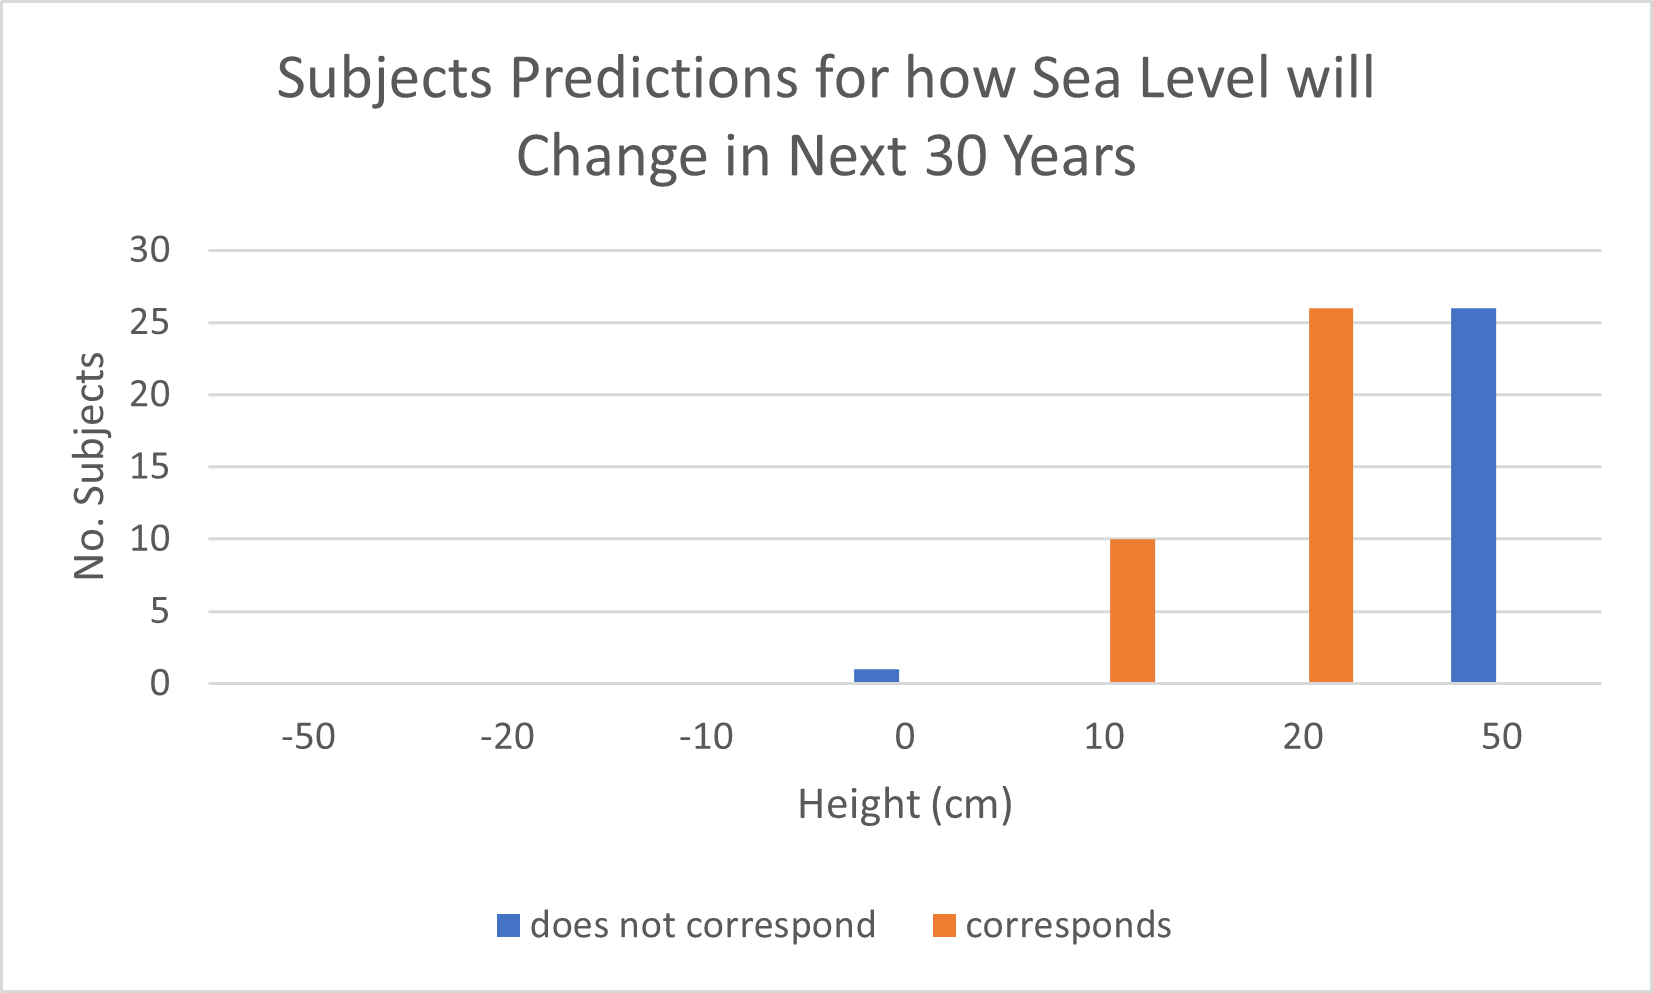
\includegraphics{fig_results/slr-future.png}
    \caption{Subjects Predictions for how Sea Level will change in Trondheim in Next 30 years. Only 147 subjects answered for this question, unlike every other one which all subjects, 153, answered. No subjects believed the sea level will decrease over the next 30 years. One subject answered that it will stay the same, with every other subject choosing that it will rise by some level }
    \label{fig:my_label}
\end{figure}

There is strong uncertainty with this measurement in models, due to the unknown of emission patterns over the next 30 years and isostatic uplift. Nevertheless, an estimation of 20cm or 10cm is in line with \cite{kartverket_se_2021} which uses the upper emissions pathways from the IPCC. Over half of the subjects chose an answer which is in line with models from \cite{kartverket_se_2021}. However, equal numbers of subjects, 26 , chose 50cm as chose 20cm,  which is not in line with these models. Almost all subjects answered that sea level will rise in the next 30 years, though six subjects chose not to answer this question.  

As shown in the survey attached in the appendix, Figure 5.21 and Figure 5.22 display results from questions which were purely numerical answers. There were no edited photographs to show the simulated SLEs.
\paragraph{}


\begin{figure}[H]
    \centering
    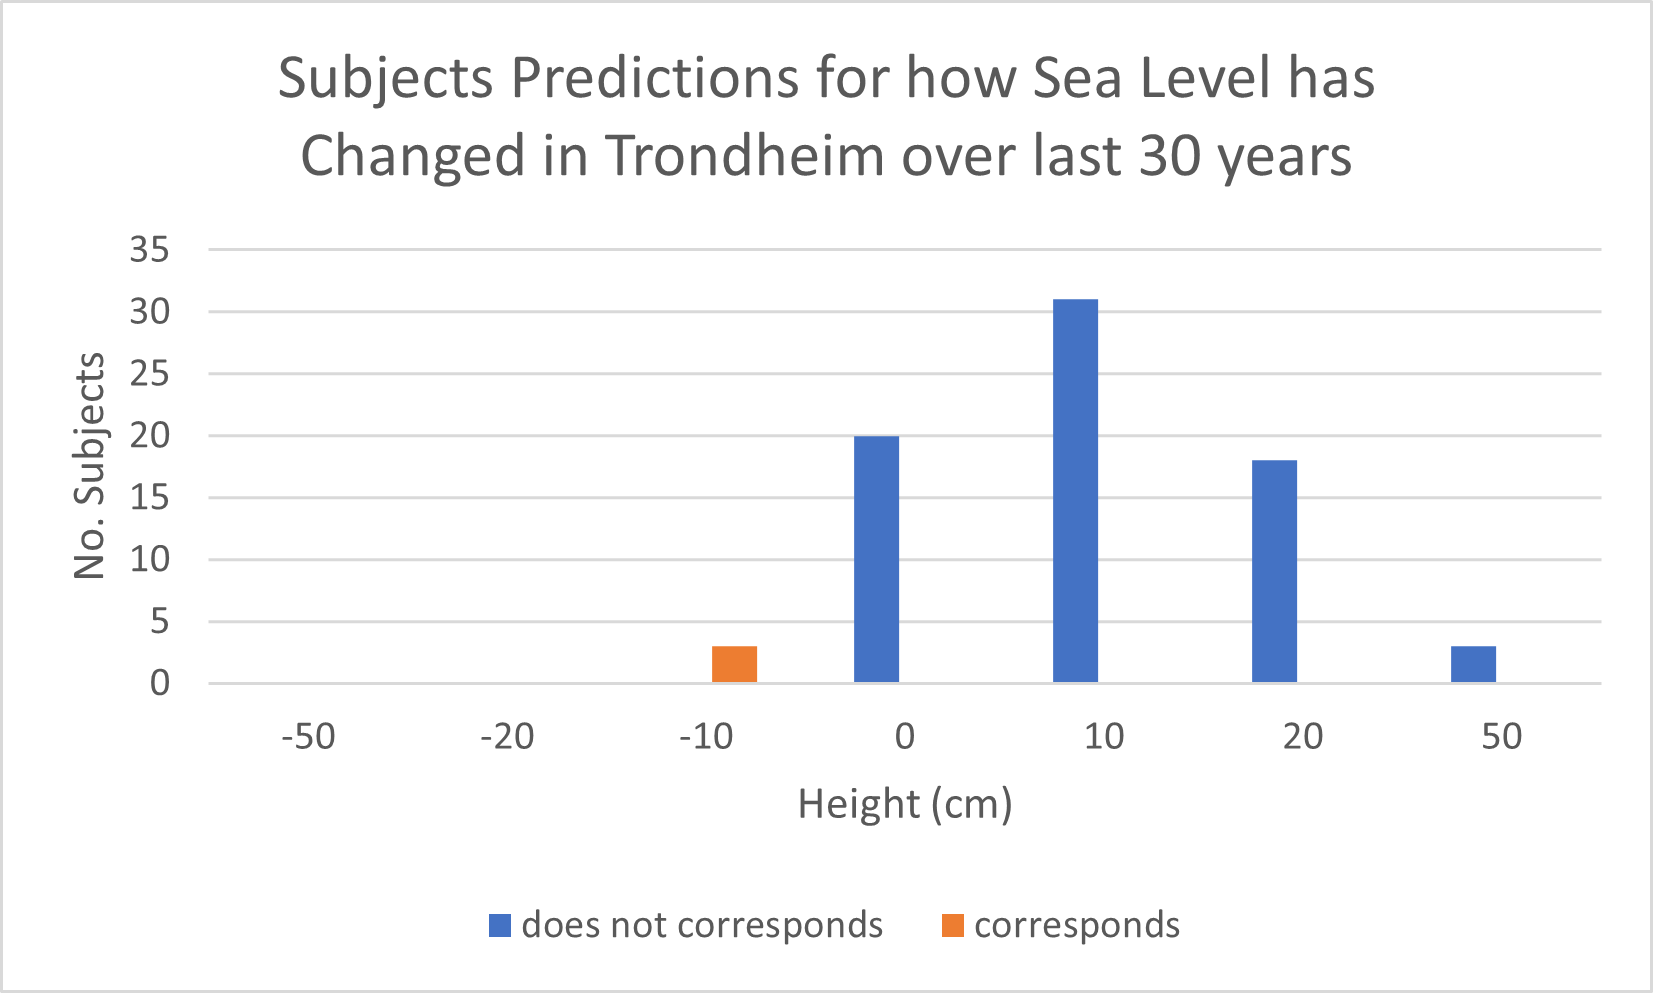
\includegraphics{fig_results/slr-past.png}
    \caption{Subjects Predictions for how Sea Level has Changed in Trondheim over last 30 years. Only 3 subjects chose that sea level has decreased in the last 30 years, this answer is inline with \cite{kartverket_se_2021}. 20 subjects answered that sea level had not changed over this time. While 31 subjects answered that it had risen by 10 cm. 18 subjects answered that it had risen by 20 cm and 3 answered that it had risen by 50 cm. 52 subjects answered that sea level had risen over the last 30 years. }
    \label{fig:my_label}
\end{figure}

Figure 5.22 shows the subjects predictions for how sea level has changed in Trondheim over the last 30 years. The certainty for the models presented here is high, as they are based off recordings not projections. 
\paragraph{}

Figure 5.23 is a combination of all results thus far in this section on awareness. This was the first attempt to determine awareness of subjects from the results of this survey

\begin{figure}[H]
    \centering
    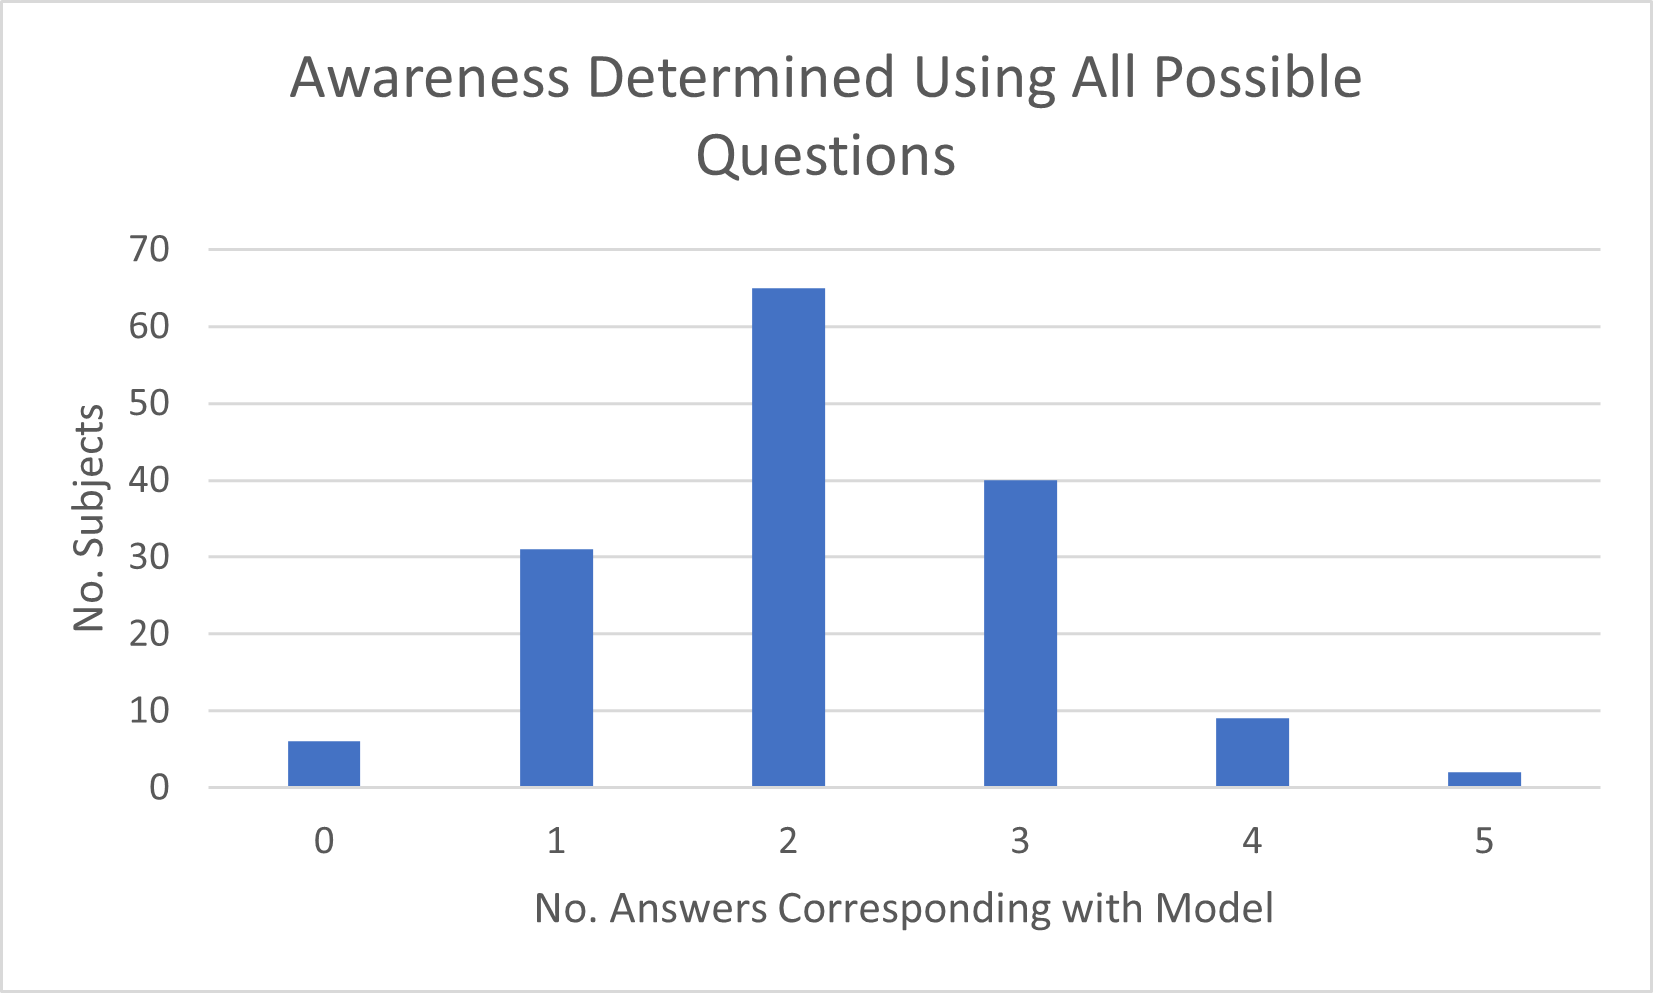
\includegraphics{fig_results/aware_all.png}
    \caption{Awareness Considering all Questions which were designed to determine awareness.  2 subjects had all answers corresponding with the models from \cite{kartverket_se_2020}. 9 subjects had 4 answers corresponding, 40 subjects had 3 answers corresponding, 65 subjects had 2 answers corresponding, 31 subjects had 1 answer corresponding and 6 subjects had no answers corresponding. }
    \label{fig:aware-all}
\end{figure}
\paragraph{}

Awareness determination considering all answers related to questions was not the most suitable for analysing factors related to awareness. For this reason, another determination of awareness was created utilising only the questions which had pictures of the simulated water levels. This is discussed further in chapter 6. 
\paragraph{}
Figure 5.24 shows determination of awareness considering the questions which utilised edited photographs, excluding the questions which were purely numeric. 

\begin{figure}[H]
    \centering
    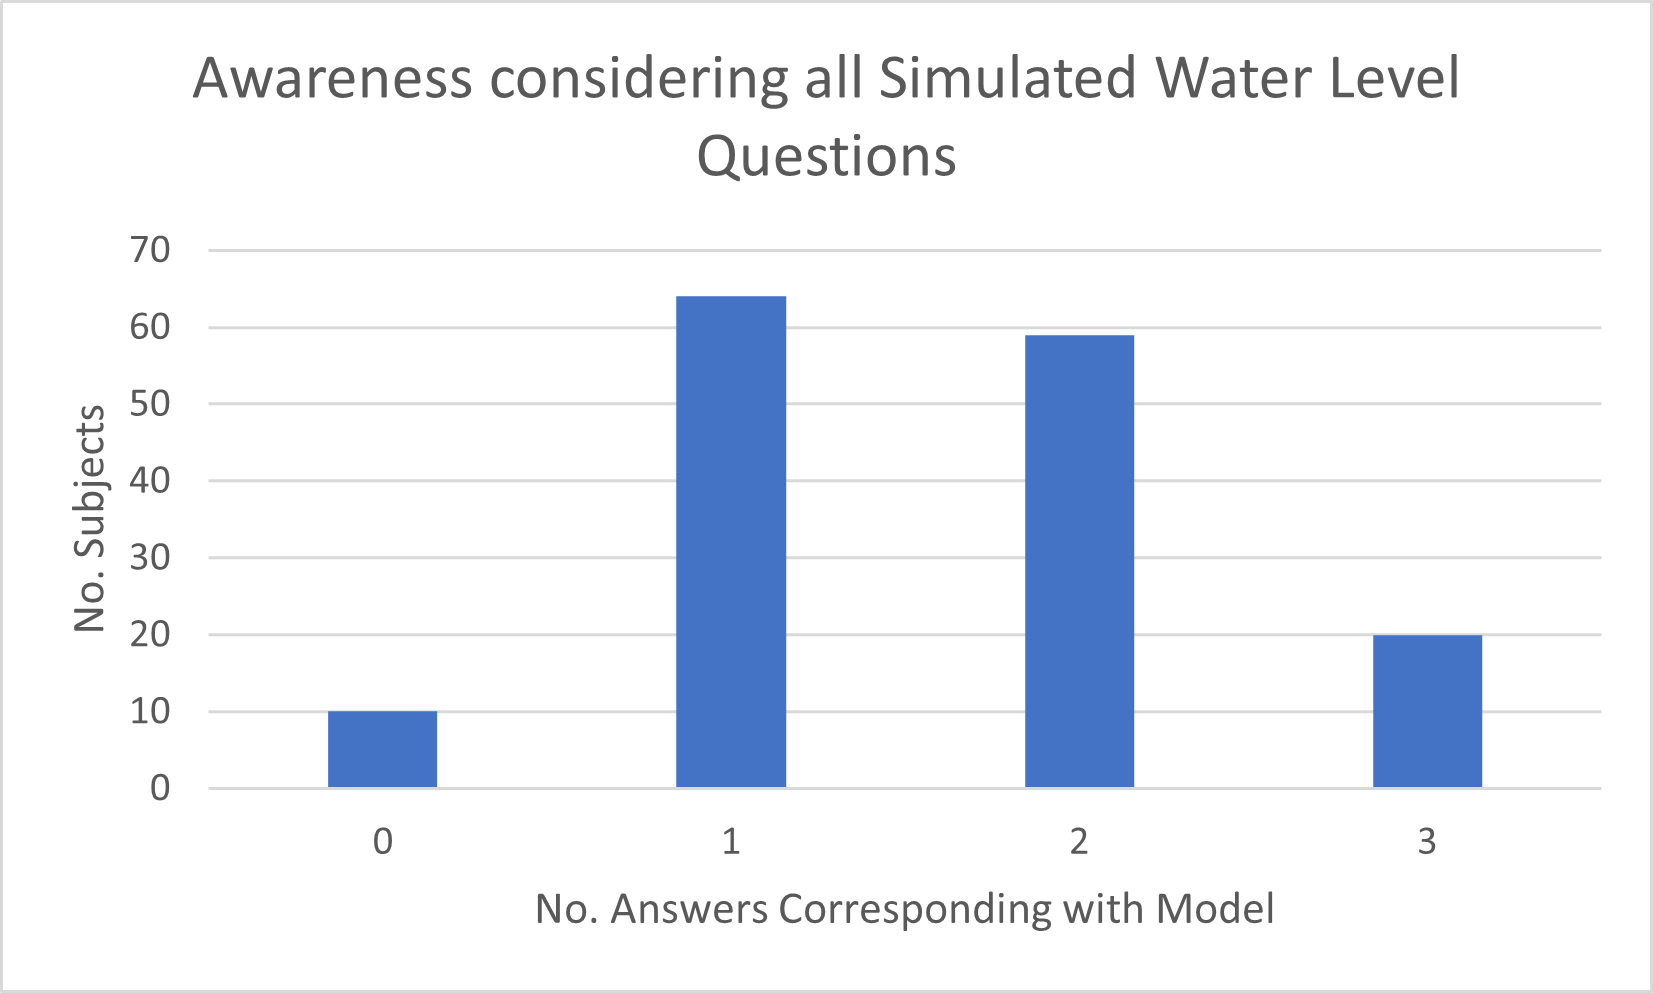
\includegraphics{fig_results/Awareness_ all_simulation_pictures_qs.png}
    \caption{Awareness considering all Visually Simulated Water Level Questions. 10 subjects had no answers corresponding with the models from \cite{kartverket_se_2020}, 20 subjects responded with every answer corresponding with the model for these questions. 64 subjects responded to one of the four questions with answers which corresponded with the models. 59 subjects responded with 2 answers which corresponded with the models. }
    \label{fig:aware_all}
\end{figure}


The results here are more evenly spread than in figure 5.23, with the majority of subjects classing as somewhat aware.
\paragraph{}
 


\paragraph{}
As shown by the focus group there is issues with just requesting a numeric value from subjects. There is a higher potential connection for many individuals including another emotional layer when using pictures rather than numbers. 

\section{Factors Affecting Awareness}
  

\subsection{Shapiro Test Results}

During histogram analysis, only the factors of "interest-level" and "info-climate-sum" appeared normally distributed. To investigate whether these factors were truly normally distributed, a Shapiro test was carried out using \cite{royston_extension_1982}.  An assumption of alpha value of 0.05 was determined meaningful (\cite{royston_extension_1982}). This means if the p-value created during this test is below 0.05 then the null hypothesis is rejected. This does leave a 5 percent chance of error. The results from the Shapiro test can be seen in Table 5.5 and this determines that none of the variables were normally distributed. 

\begin{table}[H]
    \centering
    \begin{tabular}{|l|l|l|l|}
    \hline
         \textbf{ Variable } &  \textbf{W-value}& \textbf{ P-Value}& \textbf{Distribution}\\ \hline
       Interest Level & 0.89332 & 4.343e-09 & Skewed \\ \hline
         Info Climate Sum  & 0.95721 & 0.0001159 & Skewed \\ \hline
        Flood Impact & 0.87779 & 6.681e-10 & Skewed \\ \hline
     \end{tabular}
    \caption{Shapiro Test Results. The alpha value was assigned 0.05, meaning that if the p-value is below 0.05 then the null hypothesis that this factor is not normally distributed was rejected. This leaves a 5 percent chance of error. Each of these factors p-value is below 0.05 meaning that their distribution was deemed skewed.Interest Level is when subjects self-identified their interest level in SLEs, ranging from professional interest to no interest. Info Climate Sum is the total of how many different sources subjects used to gather information about the climate. Flood impact is what the subjects predicted a flood in the place would impact them ranging from no impact to significant impact. }
    \label{table:shapiro_test_results}
\end{table}
\paragraph{}

This result that all variables and factors were skewed, including the important variable of awareness and interest level, influenced the choice of how to analyse dependency. As outlined in the method (chapter 3) Kruskal Wallis Rank Sum Tests were chosen due to the need to investigate multiple groups, upon one factor and having only measured each subject once.

\subsection{Kruskal Wallis Rank Sum Test}
The results from Kruskal Wallis Rank Sum Test conducted using the RStudio package based off \cite{hollander_nonparametric_2014} are outlined below.  An alpha value of 0.05 was chosen before these tests were carried out. This means there is a 5 percent chance of error when determining dependency of factors against the variable of awareness.
\paragraph{}
For clarity, the statistical labels for the Kruskal Wallis Rank Sum test are quickly outlined. For each of the results below, the p-value is the probability that measures the evidence against the null hypothesis.  If the p-value is lower than the selected alpha-value (0.05), then the null hypothesis can be rejected. The alternative way that the null hypothesis can be rejected utilises the H-value, which is the test statistic. If the df is over four and the h-value is particularly high this can assist in the rejection of the hypothesis. Df stands for degrees of freedom, which is the number of groups within that factor, minus one. Statistical interpretation used guidance from \cite{minitab_interpret_2022}.
\paragraph{}

Table 5.6 shows that, for the determination of awareness considering all questions on awareness, none of the factors were classed as dependent, when using the Kruskal Wallis rank sum test with an alpha value of 0.05. 

\begin{table}[H]
    \centering
    \begin{tabular}{|l|l|l|l|}
    \hline
         ~ & \textbf{awareness A} & ~ & ~ \\ \hline
        Factor & p value & h value & df \\ \hline
           length of Knowledge & 0.73760 & 3.54770 & 6 \\ \hline
       Interest Level in SLE & 0.16920 & 6.43150 & 4 \\ \hline
        Concern about Climate & \cellcolor[HTML]{7df9ff} 0.05630 & \cellcolor[HTML]{7df9ff} 9.19960 & \cellcolor[HTML]{7df9ff} 4 \\ \hline
        Language of Survey & 0.2041 & 1.6129 & 1 \\ \hline
        Predicted Personal Impact of Flood & 0.7156 & 1.357 & 3 \\ \hline
    \end{tabular}
    \caption{Kruskal Wallis Test Results General Factors. "awareness A" means that for this determination of awareness, all five questions on awareness in the survey were included. Length of knowledge is how many years the subjects state they have knowledge of the places. Interest level in SLE represents the self-ranking of subjects from professional interest to no interest. Concern about Climate is self ranking of how concerned subjects are about climate change, from one to five. Language of survey, is whether the subjects chose to respond in Norwegian or English. Predicted Personal Impact of Flood is specifically for flooding in the research place and ranges from no impact to significant impact. }
    \label{Kruskal_wallis_test_general}
\end{table}

All the p-values were larger than the alpha value of 0.05. However, the p-value of Concern about Climate is 0.05630, highlighted in blue, is only just over.  If the alpha value was chosen to be 0.1, as is used in some studies (\cite{hollander_nonparametric_2014}), then this would be enough to reject the null hypothesis that concern about awareness is not dependent upon concern about climate. However, the h-value is exceptionally high and the df is 4, meaning that, while not as confident as with a p-value rejection, the null hypothesis is still rejected (\cite{minitab_interpret_2022}). The result is that awareness appears dependent upon Concern about climate. 
\paragraph{}


Table 5.7 shows the Kruskal Wallis Test Results for the factors about the subjects community memberships. 


\begin{table}[H]
    \centering
    \begin{tabular}{|l|l|l|l|}
    \hline
         ~ & \textbf{awareness A} & ~ & ~ \\ \hline
        Factor & p value & h value & df \\ \hline
        Sum of Community Memberships & 0.52060 & 4.20260 & 7 \\ \hline
        Marine worker & na & na & na \\ \hline
        Worker & 0.12310 & 2.37220 & 1 \\ \hline
        Resident & \cellcolor[HTML]{7df9ff} 0.01524 & 5.88900 & 1 \\ \hline
        Student & 0.55590 & 0.34691 & 1 \\ \hline
        Commuter & 0.44610 & 0.58063 & 1 \\ \hline
        Leisure User Land & 0.68790 & 0.16141 & 1 \\ \hline
        Leisure User water & 0.42120 & 0.64690 & 1 \\ \hline
        Other & 0.58620 & 0.29627 & 1 \\ \hline
    \end{tabular}
    \caption{Kruskal Wallis Test Results Community Membership. "awareness A" means that for this determination of awareness, all five questions on awareness in the survey were included. Sum of Community Memberships is how many communities did the subjects select in the survey. Marine worker is whether the subject considered themselves a marine worker. This had no responses. Community memberships also included worker, resident, student, commuter, leisure user land, leisure user water and other. The Other community membership was where the subjects self-identified their community: the most common response was tourist, with sailor coming next. }
    \label{Kruskal_wallis_test_general}
\end{table}
Resident is the only value which is highlighted in Table 5.7 as it is the only significant result when utilising a alpha value of 0.05. The factor of resident has a P-value of 0.01524, meaning the differences between the medians are statistically significant. This allows the rejection of the null hypothesis and the acceptance of the positive hypothesis that awareness is dependent on residency. 
\paragraph{}

Table 5.8 shows the Kruskal Wallis Test Results on the factors covering Information Sources for Place. Two forms of determining awareness are used as predictors. "awareness A", where all five questions on awareness in the survey were included and "awareness B", where only the questions which utilised edited photographs are used to determine awareness.

\begin{table}[H]
    \centering
    \begin{tabular}{|l|l|l|l|l|l|l|}
    \hline
       & \textbf{awareness A} & ~ & ~ & \textbf{awareness B} & ~ & ~ \\ \hline
       Factor & p value & h value & df & p value & h value & df \\ \hline
        Sum of Sources  & 0.44600 & 6.85110 & 7 & 0.45040 & 6.79650 & 7 \\ \hline
        Personal Observation & 0.22730 & 1.45790 & 1 & 0.36470 & 0.82162 & 1 \\ \hline
        Family & 0.78550 & 0.07406 & 1 & 0.81340 & 0.05572 & 1 \\ \hline
        Friend & 0.27580 & 1.18780 & 1 & 0.30200 & 1.06520 & 1 \\ \hline
        Newspaper & 0.74490 & 0.10583 & 1 & 0.48500 & 0.48765 & 1 \\ \hline
        TV & 0.87330 & 0.02542 & 1 & 0.33420 & 0.93237 & 1 \\ \hline
        Social Media & 0.48540 & 0.48671 & 1 & 0.95090 & 0.00379 & 1 \\ \hline
        Membership of Organisation  & 0.67530 & 0.17550 & 1 & 0.70980 & 0.13848 & 1 \\ \hline
        Municipality & 0.82590 & 0.04839 & 1 & 0.12790 & 0.57600 & 1 \\ \hline
        \hline
    \end{tabular}
    \caption{Kruskal Wallis Test Results: Information Sources for Place as Factor.  "Awareness A" means that for this determination of awareness the three questions on awareness utilising edited photographs were included, which display awareness of the tide and present and future storm surges.  "Awareness B" excludes the future storm surge response and only considers the present storm surge and tide.  The sum of sources is the total number of sources each subject selected as where they gather information about place from. These sources are personal observation, family, friend, newspapers, TV, social media, via membership of organisations and the Municipality. }
    \label{Kruskal_wallis_test_information}
\end{table}

There were no significant values, meaning that for each of these hypotheses the null hypotheses was accepted.
\paragraph{}
Table 5.9 shows the Kruskal Wallis Test Results on the factors Information Sources for Climate. As with Table 5.8, two determinations of awareness are used as predictors.



\begin{table}[H]
    \centering
    \begin{tabular}{|l|l|l|l|l|l|l|}
    \hline
        & \textbf{awareness A} & ~ & ~ & \textbf{awareness B} & ~ & ~ \\ \hline
        Factor & p value & h value & df & p value & h value & df \\ \hline
        Sum of Sources & 0.91220 & 3.32660 & 8 & 0.45218 & 8.12040 & 8 \\ \hline
        Personal Observation & 0.11750 & 2.45020 & 1 & 0.24550 & 1.34870 & 1 \\ \hline
        Family & \cellcolor[HTML]{7df9ff} 0.00481 & 0.94470 & 1 & 0.56970 & 0.32313 & 1 \\ \hline
        Friend & 0.82460 & 0.04910 & 1 & 0.63010 & 0.23186 & 1 \\ \hline
        Newspaper & 0.09036 & 2.86790 & 1 & \cellcolor[HTML]{7df9ff} 0.01218 & 6.24830 & 1 \\ \hline
        TV & 0.61230 & 0.25689 & 1 & 0.75000 & 0.10154 & 1 \\ \hline
        Social Media & 0.74950 & 0.10960 & 1 & 0.92830 & 0.00809 & 1 \\ \hline
        Membership of Organisation & 0.30270 & 1.06220 & 1 & 0.27500 & 1.91500 & 1 \\ \hline
        Peer Reviewed Publications  & 0.88040 & 0.02650 & 1 & 0.12390 & 2.36760 & 1 \\ \hline
        Formal Education & 0.64850 & 0.20779 & 1 & \cellcolor[HTML]{7df9ff} 0.02438 & 5.06770 & 1 \\ \hline
    \end{tabular}
    \caption{Kruskal Wallis Test Results Variables on Information Sources for Climate. "Awareness A" means that for this determination of awareness the three questions on awareness utilising edited photographs were included, which display awareness of the tide and present and future storm surges.  "Awareness B" excludes the future storm surge response and only considers the present storm surge and tide.  The sum of sources is the total number of sources each subject selected as from where they gather information about changes to the climate. These sources are personal observation, family, friend, newspapers, TV, social media, via membership of organisations, peer reviewed publications and formal education. The values highlighted in blue are statistically significant. }
    \label{Kruskal_wallis_test_information}
\end{table}

For the determination of awareness which considered all five possible questions, Family is a significant factor. This means that this determination of awareness appears dependent on family as a sources of observation. This result is discussed later in the context that 25 subjects have a personal connection to the researcher.
\paragraph{}
For the determination of awareness which only utilised the edited photograph questions, both the information source of newspaper and formal education were significant.
\paragraph{}
Table 5.10 shows the Kruskal Wallis Test Results on the factors of Place subjects responded on. These places had varied physical vulnerability as outlined in Table 2.1 in the background.

\begin{table}[H]
    \centering
    \begin{tabular}{|l|l|l|l|l|l|l|}
    \hline
~ & \textbf{awareness A} & ~ & \textbf{awareness B} & ~ &  \\ \hline
        Factor & p value & h value & df & p value & h value & df\\ \hline
         Brattøra & 0.1044  & 2.6364 & 1 & 0.771 & 0.084739 &1\\ \hline
        Grillstad & 0.1815 & 1.7855 & 1 & 0.1565 & 2.008 & 1 \\ \hline
       Skansen & 0.09349 & 2.8133 & 1 & 0.05527 & 3.6738 & 1\\ \hline
         Nidelva & 0.2472 & 1.3388 & 1 & 0.9523 &  0.0035714 & 1\\ \hline
    \end{tabular}
    \caption{Kruskal Wallis Test Results: Place as Factor. "Awareness A" means that for this determination of awareness the three questions on awareness utilising edited photographs were included, which display awareness of the tide and present and future storm surges.  "Awareness B" excludes the future storm surge response and only considers the present storm surge and tide.  Brattøra, Grillstad, Skansen and Nidelva are the places considered.}
\end{table}
None of the factors of each of the places have a statistically distinct median. This means the null hypothesis is accepted and awareness is not considered dependent on the variable of place. 
  How the non-parametric hypothesis testing of Kruskal Wallis Rank Sum tests relate to the original hypotheses it outlined at the end of the discussion section.   
\paragraph{}

  









